% CURE-Rec manuscript -- Springer Nature template, empirical-result version.
% Compile from this directory with: pdflatex cure-rec; bibtex cure-rec;
% pdflatex cure-rec; pdflatex cure-rec.
% The manuscript deliberately separates controlled causal claims (CURE-Sim)
% from external chronological-ranking claims (MovieLens-1M).

\documentclass[pdflatex,sn-mathphys-num]{sn-jnl}

\usepackage{graphicx}
\usepackage{multirow}
\usepackage{amsmath,amssymb,amsfonts}
\usepackage{amsthm}
\usepackage{mathrsfs}
\usepackage[title]{appendix}
\usepackage{xcolor}
\usepackage{textcomp}
\usepackage{manyfoot}
\usepackage{booktabs}
\usepackage{tabularx}
\usepackage{algorithm}
\usepackage{algpseudocode}
\usepackage{array}
\usepackage{url}
\usepackage{hyperref}
\usepackage{tikz}
\usetikzlibrary{positioning,arrows.meta}

\theoremstyle{thmstyleone}
\newtheorem{theorem}{Theorem}
\newtheorem{proposition}[theorem]{Proposition}
\newtheorem{corollary}[theorem]{Corollary}
\theoremstyle{thmstyletwo}
\newtheorem{example}{Example}
\newtheorem{remark}{Remark}
\theoremstyle{thmstylethree}
\newtheorem{definition}{Definition}

\newcommand{\Players}{\mathcal{N}}
\newcommand{\Models}{\mathcal{M}}
\newcommand{\Policy}{\pi}
\newcommand{\BasePolicy}{\pi_0}
\newcommand{\Utility}{V}
\newcommand{\Shap}{\phi}
\newcommand{\E}{\mathbb{E}}
\newcommand{\R}{\mathbb{R}}
\newcommand{\NDCG}{\mathrm{NDCG@10}}
\newcommand{\Recall}{\mathrm{Recall@10}}
\newcommand{\CURE}{\textsc{CURE-Rec}}
\newcommand{\Sim}{\textsc{CURE-Sim}}

\raggedbottom

\begin{document}

\title[CURE-Rec]{CURE-Rec: Exact Cooperative Games over Policy Interventions for Robust Policy Selection in Sequential Recommendation}

\author*[1]{\fnm{Mouad} \sur{Louhichi}}\email{mouad\_louhichi@um5.ac.ma}
\author[1]{\fnm{Redwane} \sur{Nesmaoui}}\email{redwane\_nesmaoui@um5.ac.ma}
\author[1]{\fnm{Mohamed} \sur{Lazaar}}\email{mohamed.lazaar@ensias.um5.ac.ma}
\affil*[1]{\orgdiv{National Higher School of Computer Science and Systems Analysis (ENSIAS)}, \orgname{Mohammed V University in Rabat}, \orgaddress{\city{Rabat}, \country{Morocco}}}

\abstract{Recommendation interventions change the exposure process that generates future feedback, yet systems commonly choose exploration, diversity, long-tail, repetition-control, and provider-balancing policies from local ranking metrics or isolated ablations. Those choices are difficult because interventions overlap, conflict, incur costs, and may be required to repair a constraint-infeasible base policy even when their short-run utility increment is small. We introduce \CURE{}, a decision layer that treats a bounded library of feasible policy transformations as players in an exact cooperative game. The game is evaluated under disclosed sequential recommendation scenarios, attributed by Shapley values and pairwise interactions, and optimized directly under relevance, fatigue, provider-disparity, and budget constraints. The planner distinguishes improvement from repair: it may retain a feasible base policy when no portfolio robustly improves it, selects the best feasible repair when the base violates a constraint and a feasible repair exists, and otherwise reports that no feasible portfolio is available. We validate the framework in controlled oracle regimes, a behavioural sequential benchmark, one-at-a-time and joint Latin-hypercube robustness studies, and a separate real-data ranking evaluation. In the full 20-seed behavioural study, repeated-exposure control is selected in all seeds with a mean robust lower improvement of $0.29371$ (standard deviation $0.00258$) on the normalized CURE-Sim utility scale. Joint calibration reveals documented switches, induced by changing feasibility and scenario assumptions, to provider balancing, complementary portfolios, and abstention. We additionally report held-out selector comparisons on configurations in which the exact planner and simpler selectors choose different portfolios---where the exact constrained planner achieves the best held-out robust value in 20 of 20 evaluation seeds---sensitivity analyses over the normative utility weights and the constraint surface, and a semi-real integration in which a BPR-MF ranker trained on simulator-logged feedback serves as the base policy inside the intervention game with a consistent decision. On MovieLens-1M, under identical warm-item candidates and audit checks, frozen SASRec reaches $\Recall=0.1452\pm0.0031$ and $\NDCG=0.07424\pm0.00281$ across five seeds, versus popularity's $0.049$ and $0.02552$. This real-data experiment validates the shared chronological ranking/evaluation pipeline and the implemented rankers; it does not validate the \CURE{} portfolio-selection layer and is not a causal policy-effect claim. Additional approximation, CRN, scalability, and second-dataset analyses are reported as bounded robustness-probing evidence rather than causal policy claims.}

\keywords{Recommender systems, Explainable AI, cooperative games, Shapley value, policy intervention, multi-stakeholder recommendation, robust optimization, sequential decision making, constrained recommendation}

\maketitle

\section{Introduction}\label{sec:introduction}

Recommendation is not only prediction. From the earliest collaborative-filtering systems \cite{resnick1994grouplens,sarwar2001item,linden2003amazon} to modern industrial retrieval-and-ranking pipelines \cite{covington2016youtube,ricci2015recommender}, a deployed policy decides which items receive exposure, exposure changes short-term response and repeated-item fatigue, and the resulting feedback modifies the popularity and behavioural signals used at later decisions. The operational question is therefore not only which item should be ranked first at a single time point. It is also which feasible part of the policy should be changed when the current system over-repeats items, under-serves providers, over-concentrates attention, or fails to explore. Production teams already manipulate repetition caps, exploration slots, long-tail promotion, diversity rerankers, novelty slots, and provider balancing \cite{castells2015novelty,abdollahpouri2019popularity,burke2018multistakeholder}. What is generally missing is a coherent way to evaluate their joint long-term consequences and to allocate credit when several interventions are redundant or antagonistic.

A common response is an isolated ablation: activate one intervention, compare a metric with the base policy, and retain the intervention that appears best. Such one-at-a-time evidence is widespread in industrial reporting and in the academic literature on individual re-ranking objectives \cite{ziegler2005improving,vargas2011rank,abdollahpouri2019popularity}. It is, however, a weak basis for a portfolio decision. An exploration slot may be useful only after a repeat cap releases a position; long-tail and novelty slots can compete for the same bounded insertion capacity; a provider correction may be warranted because the base policy violates a platform constraint even if it does not maximize an unconstrained utility increment. Isolated effects do not sum to the value of a portfolio, and a high attribution score alone does not identify a feasible decision.

More precisely, several capabilities are typically absent \emph{jointly} from existing approaches, rather than each being absent from every approach. Table~\ref{tab:capability-gap} summarizes the gap that motivates this work: coalition-level interaction modelling under a shared long-horizon environment, hard feasibility constraints, explicit repair semantics when the base policy is constraint-infeasible, and exact rather than sampled attribution. \CURE{} combines these capabilities for a bounded intervention library; it does not claim that any single ingredient is new.

\begin{table*}[t]
\caption{Capabilities required for portfolio-level intervention decisions. ``Partial'' indicates that the capability exists only for single interventions, single metrics, or sampled approximations in the cited lines of work. This paper combines all five capabilities for a bounded intervention library.}\label{tab:capability-gap}
\centering
\small
\setlength{\tabcolsep}{4pt}
\begin{tabularx}{\textwidth}{@{}p{0.30\textwidth}ccccc@{}}
\toprule
Approach family & Coalition interactions & Long horizon & Hard constraints & Repair semantics & Exact attribution\\
\midrule
Isolated ablations / single-objective reranking \cite{ziegler2005improving,vargas2011rank,abdollahpouri2019popularity} & No & Partial & No & No & No\\
Multi-stakeholder and fairness reranking \cite{burke2018multistakeholder,singh2018fairness,ekstrand2022fairness} & Partial & Partial & Partial & No & No\\
Off-policy and counterfactual evaluation \cite{swaminathan2015counterfactual,joachims2017unbiased,kallus2020efficient} & No & Yes & Partial & No & No\\
Feature/data Shapley attribution \cite{lundberg2017shap,mcelfresh2023shapley} & Partial & No & No & No & Sampled at scale\\
\CURE{} (this paper, bounded library) & Yes & Yes & Yes & Yes & Yes\\
\bottomrule
\end{tabularx}
\end{table*}

\CURE{} addresses this gap with a small, exact cooperative game over \emph{policy interventions}. Its six players are predeclared slate transformations rather than users, items, model features, or arbitrary retraining operations. A coalition applies a deterministic canonical composition to a fixed base policy. For each coalition and each disclosed sequential scenario, \Sim{} rolls out a finite-horizon platform process with preference, popularity feedback, repeated exposure, fatigue, novelty, and provider exposure. The resulting coalition values support exact Shapley attribution, exact pairwise interaction analysis, and a direct robust portfolio decision. Attribution explains a decision; it never replaces the decision rule.

The paper makes four contributions.
\begin{enumerate}
\item \textbf{A decision-facing cooperative game over feasible policy changes.} We formalize a fixed intervention library, exact collision semantics for competing injection interventions, scenario-indexed coalition values, Shapley regions, and interaction regions. The six-player library induces only $2^6=64$ coalitions, making exact rather than sampled attribution practical. Exactness is not claimed as the principal contribution by itself: it is a deliberate consequence of bounding the intervention library, and it is what allows the decision machinery below to be audited without Monte-Carlo attribution error.
\item \textbf{Robust improvement and repair semantics.} We formulate a constrained direct portfolio optimizer that distinguishes a constraint-feasible base policy from a constraint-infeasible one. In improvement mode it can abstain; in repair mode it must select the best feasible portfolio or report that none exists. This separation prevents a negative utility difference from being misread when an intervention is needed to restore constraint feasibility.
\item \textbf{Controlled and behavioural evidence.} Nine analytic oracle regimes test additive, complementary, redundant, antagonistic, delayed, repair, and misspecified settings. A 20-seed behavioural study, a 15-point one-at-a-time study, and a 25-point joint Latin-hypercube study test whether the decision pattern survives disclosed changes in horizon, fatigue, repetition, provider constraints, novelty benefit, intervention strength, and intervention cost. Complementary revision experiments test the decision itself: held-out selector comparisons in configurations where simpler selectors disagree with the exact planner, a sensitivity sweep over the normative utility weights, and a phase diagram of the decision over the joint constraint frontier.
\item \textbf{A separately audited real-data robustness protocol.} We evaluate popularity, BPR-MF, and SASRec on MovieLens-1M using the same chronological split, warm-item candidate set, cold-target accounting, validation-only configuration selection, final audit, and fixed-configuration seed replication. This establishes ranking robustness of the implementation while preserving the boundary that MovieLens is not a complete causal policy log.
\end{enumerate}

The central claim is deliberately bounded. \CURE{} provides causal-oracle and behavioural claims inside \Sim{}, where the sequential data-generating mechanisms and intervention values are disclosed. It provides real-data ranking claims on MovieLens-1M under an audited evaluator. It does not claim that MovieLens identifies the long-run causal effects of production policy changes: it contains neither logged slates, exposure propensities, nor a complete candidate-set record. This separation is a methodological requirement rather than a limitation hidden in the evaluation.

\section{Literature review}\label{sec:literature}

\subsection{Recommendation as a sequential intervention problem}

Collaborative filtering and sequential recommendation are usually introduced as supervised ranking problems, from probabilistic and regularized matrix factorization \cite{mnih2008probabilistic,koren2009matrix} and Bayesian personalized ranking \cite{rendle2009bpr,pan2008oneclass} to neural collaborative filtering \cite{he2017ncf}, recurrent and self-attentive sequence models \cite{hidasi2016gru,kang2018sasrec,sun2019bert4rec}, and graph-based methods \cite{wang2019ngcf,he2020lightgcn}. These models are powerful predictors, but prediction quality does not by itself decide whether a platform should increase exploration, reduce repetition, or rebalance exposure. A recommendation is an action that changes the observations on which future training and ranking depend. This closed loop motivates causal recommender work and counterfactual learning-to-rank \cite{swaminathan2015counterfactual,joachims2017unbiased,wang2023causal,bonner2018causal}; recent surveys systematize this literature and its identification requirements \cite{gao2024causal}. A complementary recent line studies how recommendation feeds back into the ecosystem itself: user--creator feature dynamics can polarize under dual influence \cite{lin2024polarization}, exploration mediates a trade-off between short-run user satisfaction and long-run creator productivity \cite{yao2024satisfaction}, and platform participants can strategically act on the training data \cite{baumann2024collective}. These results reinforce the premise of the present paper---exposure decisions have long-horizon, multi-sided consequences---while also illustrating why finite-horizon simulator evidence must be labelled as such: our behavioural benchmark discloses one concrete feedback mechanism and does not model strategic creators.

The available evidence often limits what can be inferred. Observational ratings typically record a response but not the alternatives shown, the rank at which they were shown, the logging probability, or the contemporaneous candidate set \cite{pearl2009causality,athey2017state}. Treating such records as complete randomized policy logs conflates preference, exposure, and selection. Work on recommendation as treatment makes this distinction explicit \cite{schnabel2016recommendations}; doubly robust and sequential off-policy approaches require the logging information that ordinary ratings files lack \cite{dudik2014doubly,kallus2020efficient}. \CURE{} follows that discipline: the causal intervention game is tested in an oracle benchmark; the MovieLens experiment remains a separate chronological-ranking robustness evaluation.

\subsection{Diversity, novelty, repetition, and provider exposure}

A long literature improves recommendation lists through diversity, novelty, long-tail exposure, popularity-aware reranking, and multi-stakeholder objectives \cite{ziegler2005improving,vargas2011rank,castells2015novelty,abdollahpouri2019popularity,burke2018multistakeholder,ekstrand2022fairness}. Recent work formalizes the multi-sided dimension of these objectives: item--user fairness can be interpolated through constrained optimization \cite{chen2024interpolating}, and user--item fairness trade-offs admit explicit frontier analyses \cite{greenwood2024fairness}. These contributions usually define one target metric or one re-ranking objective. The operational challenge is that their transformations can collide. A diversity reranker can alter the positions available to a long-tail slot; a novelty slot and a tail slot may propose the same item; and provider balancing can reduce disparity while changing relevance or fatigue. The present work does not replace those objectives. It offers a framework for assessing the exact value of their feasible combinations under a shared platform utility and explicit constraints.

The scope is intentionally modest. The intervention library is not learned from data, and it does not enumerate arbitrary changes to model architecture, user interfaces, retrieval systems, or incentives. These changes would make a coalition ill-defined and destroy exact tractability. Instead, the players are a small set of deployable slate-level transformations with clear costs and collision rules.

\subsection{Cooperative attribution and interactions}

Shapley values provide the unique cooperative allocation satisfying efficiency, symmetry, dummy, and additivity axioms \cite{shapley1953}. They have become central to feature attribution \cite{lundberg2017shap,sundararajan2017axiomatic,covert2021understanding} and to broader data and component valuation problems \cite{mcelfresh2023shapley}. When the player set is large, sampling estimators are commonly required \cite{castro2009polynomial}; the bounded intervention library lets us avoid that approximation. Their use does not make an attribution a decision: an intervention with a positive Shapley value can still be infeasible, redundant with a lower-cost substitute, or inappropriate when the base policy is already safe. We therefore use exact Shapley values as explanations of coalition values and pair them with direct constrained optimization.

Pairwise interaction measures make the non-additivity visible. The Grabisch--Roubens interaction index distinguishes complementary and antagonistic pairs \cite{grabisch1999interaction}; multilinear cooperative extensions offer related representations of coalition effects \cite{owen1972multilinear}. This is particularly relevant for policy transformations because slots and rerankers are not independent switches. The game is exact here because six interventions yield 64 coalitions per scenario. No Monte-Carlo attribution error is required. When player sets are large, exact enumeration is no longer possible and recent estimators approximate any-order Shapley interactions through weighted least squares or stratified subset sampling \cite{fumagalli2024kernelshapiq,kolpaczki2024svarmiq}; those approximation tools address precisely the regime that the bounded intervention library avoids, and they are the natural route to extending the present framework to larger libraries.

\subsection{Robust decision making under model ambiguity}

Partial-identification and robust-decision traditions caution against optimizing a single convenient causal model when several data-generating mechanisms remain plausible \cite{manski2003partial,rosenbaum2002observational,athey2017state}. In recommender systems, ambiguity can arise from fatigue strength, popularity feedback, delayed novelty benefit, provider exposure dynamics, and policy shift. \CURE{} operationalizes this caution as a finite, disclosed scenario set in the current framework. For a coalition, the relevant object is a lower utility improvement over scenarios, not a point estimate from a favourable scenario. This is an ambiguity stress test, not a claim that a finite scenario ensemble nonparametrically identifies a real-world causal effect.

\subsection{From attribution to deployment planning}

Attribution and deployment solve different optimization problems. An attribution method asks how a specified value should be divided among contributors. A deployment planner asks which action should be taken subject to operational constraints. Confusing the two creates a subtle form of overclaiming. A Shapley value can assign positive credit to an intervention because it improves some coalitions, while a planner should reject it because its cost exceeds a budget, it is redundant with a lower-cost substitute, or it makes a provider-disparity or relevance constraint fail. Conversely, an intervention may be selected as a repair even when its unconstrained utility increment is not the largest, because the current policy is not admissible.

This distinction has precedent in constrained and multi-objective recommendation, where fairness or business requirements are enforced as explicit constraints rather than as attribution scores \cite{wu2023multifr,chen2024interpolating}, but it is rarely made explicit in explanation pipelines. A common practice is to report feature or component importance and then make an informal design recommendation. That recommendation may be reasonable, but its feasibility conditions are usually outside the formal object being evaluated. \CURE{} makes the decision object explicit. The cooperative game produces a complete attribution and interaction report; the planner separately evaluates the same coalition values against declared constraints. The result is more falsifiable: a reader can inspect whether a selected portfolio was truly feasible and whether an alternative had a higher lower utility but failed a constraint.

There is also a practical reason to preserve the separation. Platform constraints differ across deployments. A provider-disparity threshold, intervention budget, or tolerated relevance change may be set by policy, product, or law rather than by a statistical estimator \cite{singh2018fairness,biega2018equity,ekstrand2022fairness,mehrabi2021survey,ge2020causal}. Re-running a small exact game with a changed constraint is transparent; retraining an opaque attribution model or quietly changing a scalarized objective is not. The calibration results in this paper are therefore not merely an uncertainty appendix. They show how the proposed decision changes when the stated operating assumptions change.

\subsection{Evaluation discipline for recommender claims}

Ranking results can be invalidated by small protocol differences, including missing-not-at-random feedback and post-selection evaluation bias \cite{yang2018unbiased,sun2020debiased,cawley2010selection}. Models may receive different candidate sets, test targets may be inadvertently removed as ``unavailable'', seen items may leak into one model's candidates, or a test result may select an epoch or a blend. These problems are especially easy to miss in a comparison between a non-personalized baseline, a matrix-factorization model, and a sequential neural model because their natural implementations expose different interfaces.

The external protocol in this paper fixes the candidate universe before model scoring, following the principle that offline ranking comparisons must not change the retrieval ceiling across methods \cite{cremonesi2010performance,harper2015movielens}. A candidate set contains warm catalogue items not seen by the user in training. All models score exactly this vector; a cold target is counted explicitly rather than converted into an apparently easier warm ranking task. Validation and test are separated: Stage A and Stage B model search write validation rows, the selected configuration is frozen in a manifest, and final test audit is run only after selection. The audit then records candidate cardinalities, target presence, score ordering, pairwise preference checks, and restored checkpoint state. This discipline is not a claim that one benchmark establishes general recommender superiority. It is the minimum required for a credible narrow claim about the implemented comparison.

The same discipline applies to uncertainty. Five seeds are useful for revealing optimization instability and for reporting a range, but they are not five independent real-world datasets. The paper reports means, sample standard deviations, minima, maxima, and paired differences rather than presenting a seed average as a universal effect size. The behavioural studies likewise report all OAT and LHS configurations rather than selecting the ones that favour the proposed planner.

\subsection{Positioning}

\CURE{} differs from conventional re-ranking in its unit of analysis: it evaluates interventions and portfolios rather than individual items. It differs from feature attribution in its players and output: the players are feasible policy changes and the output includes a robust constrained decision. It differs from off-policy evaluation because its primary causal evidence is a controlled sequential oracle environment rather than an assertion that an incomplete ratings dataset identifies a counterfactual policy value. Finally, it differs from a new base-recommender paper: the same intervention-game layer can in principle sit above a transparent simulated policy, BPR-MF, or SASRec, provided that the intervention semantics and evaluation protocol are fixed. We are explicit about the boundary of the current evidence. Section~\ref{sec:semireal} demonstrates one integrated setting---a BPR-MF ranker trained on simulator-logged feedback serving as the base policy inside the intervention game---and shows that the decision layer is consistent across the hand-crafted and learned base policies. The external MovieLens models are audited separately under the ranking protocol of Section~\ref{sec:results}; placing a ranker trained on external data inside the sequential environment remains future work.

\section{Background and preliminaries}\label{sec:background}

\subsection{Sequential recommendation environment}

Let $\mathcal{U}$ be a user cohort of $|\mathcal{U}|$ users, $\mathcal{I}$ an item catalogue of $|\mathcal{I}|$ items with provider map $\mathrm{prov}:\mathcal{I}\to\mathcal{P}$, $d$ the latent dimension, and $t\in\{0,\ldots,T-1\}$ a decision time. The platform state is
\begin{equation}
 X_t=(P_t,H_t,F_t,Q_t,E_t),
\label{eq:state}
\end{equation}
where $P_t\in\mathbb{R}^{|\mathcal{U}|\times d}$ is the public profile available to the policy, $H_t\in\mathbb{R}^{|\mathcal{U}|\times d}$ denotes latent preference state used only by the simulator response mechanism, $F_t\in[0,1]^{|\mathcal{U}|}$ is user fatigue, $Q_t\in\mathbb{R}_{\geq0}^{|\mathcal{I}|}$ is item popularity state (cumulative provider exposure is tracked alongside it in $\mathbb{R}_{\geq0}^{|\mathcal{P}|}$), and $E_t\in\mathbb{N}^{|\mathcal{U}|\times|\mathcal{I}|}$ is per-user exposure history. A base policy $\BasePolicy$ returns a ranked slate from a candidate catalogue. The environment then produces response and transition variables,
\begin{equation}
 L_t\sim \Policy(X_t),\qquad Y_t\sim p_m(Y_t\mid X_t,L_t),\qquad X_{t+1}=F_m(X_t,L_t,Y_t,\epsilon_t),
\label{eq:transition}
\end{equation}
for scenario $m\in\Models$. The notation makes clear that a policy change affects both immediate response and later state.

A clarification of the $\sim$ notation is important for the exactness claims below. In the implemented benchmark, the base policy and every coalition transformation are \emph{deterministic conditional on the observable state and a keyed random seed}: for seed $z$, the executed slate is $L_t=\Policy_S(X_t;z)$, and all simulator randomness $\epsilon_t$ (initialization, response draws, tie-breaking perturbations) is drawn from an event-indexed stream keyed by $(z,m,t,u,\mathrm{event})$. The distributional notation in Eq.~\eqref{eq:transition} therefore describes the \emph{class} of environments the framework targets; within one seed, policy stochasticity and simulator stochasticity both resolve to the keyed stream, which is what makes coalition values reproducible and coalition semantics permutation-invariant. A deployment that adds genuine policy stochasticity (for example, randomized slate sampling) would draw it from the same keyed construction; the definitions below do not otherwise change.

The behavioural benchmark uses a cohort-level process with hidden affinity, public-profile noise, repeated exposure, satisfaction-mediated preference drift, item-popularity feedback, and provider exposure. The base ranker uses public-profile similarity and popularity rather than hidden interest. This preserves a meaningful gap between the policy's information and the simulator's outcome mechanism.

Two features of this formulation matter for interpretation. First, the state is not merely an enlarged feature vector. Exposure and provider counts are shared, evolving variables: changing one user's slate can alter the popularity signal used in later ranking and the aggregate provider-disparity outcome. We consequently evaluate a cohort rollout rather than treating each user--item record as an independent supervised observation. Second, the latent-interest component is deliberately hidden from the policy. A policy that could inspect the simulator's response state would turn the benchmark into an oracle ranker and would make intervention results difficult to interpret. The policy receives only public profiles, exposure history, candidate availability, and the current popularity state.

The temporal horizon has a direct scientific role. A short horizon emphasizes the immediate relevance cost of an intervention; a longer horizon can reveal an effect operating through fatigue reduction, provider exposure, or preference drift. This is why horizon is not selected from the outcome but varied explicitly in the calibration studies. The OAT study demonstrates this distinction directly: lowering the horizon to eight reduces the mean robust lower improvement to $0.14397$, while increasing it to sixteen raises it to $0.37785$. A one-step ranking evaluation cannot express this trade-off.

\subsection{Evidence, interventions, and causal scope}

A causal claim needs more than a timestamped interaction table. For a real policy evaluation, the analyst would need at least the candidate set available at each decision, the displayed slate and positions, the logging or assignment probability, policy identifiers, a representation of eligibility and inventory, and outcomes at the time scale of the claimed effect. Without these fields, the observed response is confounded by which alternatives were exposed and by which policy generated the exposure. The absence of these fields is not repaired by fitting a more flexible predictor.

This paper therefore uses three evidence layers. The first is an \emph{analytic oracle} layer, where coalition values and true optima are defined transparently. The second is a \emph{behavioural oracle} layer, where the sequential mechanisms in Eqs.~\eqref{eq:state}--\eqref{eq:transition} generate the long-run outcome. The third is an \emph{external ranking} layer, where MovieLens-1M checks the recommender training and evaluation protocol. The layers complement one another but are not interchangeable. Controlled oracle evidence tests whether the cooperative and decision machinery reacts correctly to known structures. Behavioural evidence tests whether those mechanisms remain meaningful under feedback and fatigue. External ranking evidence tests whether the trained ranking models improve an audited held-out metric. Only the first two layers support the paper's causal intervention statements.

The player definition is also causal in a restricted but operational sense. A player is a policy transformation that can be applied while holding the base policy, candidate universe, and intervention semantics fixed. We do not define players as arbitrary features that happen to correlate with response, nor as unrestricted retraining operations. This restriction makes the intervention $do(\Policy\leftarrow\Policy_S)$ interpretable: the system replaces the deployed slate transformation with a declared alternative and executes the same sequential environment. It also makes negative results interpretable. If an intervention has no eligible candidate at a time step, it performs no operation and the event is logged. A no-op is not silently converted into another intervention.

\subsection{Policy transformations as players}

The player set is
\begin{equation}
 \Players=\{\texttt{repeat\_cap},\texttt{explore\_slot},\texttt{tail\_slot},\texttt{diversify},\texttt{novel\_slot},\texttt{provider\_balance}\}.
\label{eq:players}
\end{equation}
A coalition $S\subseteq\Players$ is a policy transformation, not a set of independently trained models. To avoid permutation-dependent semantics, every coalition follows one canonical order: repeated-exposure cap, eligibility filtering, injection allocation, diversity re-ranking, and provider balancing. The three injection players jointly compete for a capacity of two positions. Each proposes eligible items, normalizes its proposal score within its own scale, and an exact small assignment resolves collisions. A player with no eligible proposal is recorded as a no-op rather than being silently replaced by a popular item.

This design is important for interpretability. If intervention order changes with Shapley permutations, the same coalition can represent several different policies, making the characteristic function undefined. Shapley permutations average marginal contributions over set order; they must not change the operational definition of a set.

\begin{table*}[t]
\caption{Intervention players, declared membership costs, and fixed operational semantics. Costs and thresholds are configuration values rather than learned coefficients; costs are charged whenever a player belongs to the coalition, including steps at which the player records a no-op (Definition~\ref{def:cost}).}\label{tab:players}
\centering
\small
\setlength{\tabcolsep}{3pt}
\begin{tabularx}{\textwidth}{@{}p{0.14\textwidth}c X X@{}}
\toprule
Player & Cost $c_i$ & Slate transformation & Interaction and feasibility relevance\\
\midrule
Repeat cap & 0.05 & Moves items whose user-specific exposure count reaches the declared cap behind eligible alternatives. & Releases repeatedly occupied positions; can reduce fatigue and alter the feasibility of other slots.\\
Exploration slot & 0.10 & Proposes low-exposure candidates and competes for an injection position. & Has a bounded slot cost; may be complementary to repeat control or costly in relevance.\\
Long-tail slot & 0.08 & Proposes candidates below a configured popularity quantile. & Shares injection capacity with exploration and novelty; can alter provider and catalogue exposure.\\
Diversity reranker & 0.06 & Greedily reranks a bounded candidate prefix using category novelty. & Has no reserved slot but can change the slate into which injection proposals are placed.\\
Novelty slot & 0.08 & Proposes items sufficiently dissimilar from a user's public profile. & Can trade immediate relevance for delayed preference broadening in scenarios where that mechanism is active.\\
Provider balance & 0.12 & Reranks toward under-exposed providers using aggregate exposure. & Directly targets provider disparity and may be selected as a repair of a constraint-infeasible base policy.\\
\bottomrule
\end{tabularx}
\end{table*}

A coalition is consequently more than a binary feature mask. It specifies a feasible composition with a capacity constraint, eligibility rules, a tie-breaking convention, and a cost. The distinction becomes important in the LHS study. A switch from repeat cap to provider balancing is not interpreted as instability of an arbitrary score; it is an explicit response to a joint configuration in which provider feasibility, horizon, and the competing intervention costs change the robust portfolio.

\subsection{Collision allocation and policy determinism}

The three slot interventions cannot each reserve an independent position. Let
\begin{equation}
 J_S=S\cap\{\texttt{explore\_slot},\texttt{tail\_slot},\texttt{novel\_slot}\}
\label{eq:injection-set}
\end{equation}
denote the injection players active in coalition $S$. For $i\in J_S$, let $C_i(X_t)\subseteq\mathcal{I}$ be its eligible item proposals (candidates below the configured popularity quantile for tail, candidates with public-profile similarity at or below the novelty threshold for novelty, and low-exposure candidates for exploration) and $b_i(j)$ its native score for item $j$. Native uncertainty, tail-popularity, and novelty-distance scores have incompatible units, so the implementation converts each score to a within-player percentile: proposals are ranked by ascending raw score with ties broken by ascending item identifier, and a proposal with rank $r\in\{0,\ldots,|C_i|-1\}$ receives
\begin{equation}
 \widetilde b_i(j)=\frac{r(j)+1}{|C_i(X_t)|}\in(0,1].
\label{eq:percentile}
\end{equation}
This tie rule is deterministic and identical across coalitions, so the normalized score never depends on attribution order. With capacity $q=2$, the selected assignment is
\begin{equation}
 \max_{x}\ \sum_{i\in J_S}\sum_{j\in C_i(X_t)}\widetilde b_i(j)x_{ij}
\quad\text{s.t.}\quad
\sum_{j\in C_i(X_t)}x_{ij}\leq1\ \forall i,\quad
\sum_{i\in J_S}x_{ij}\leq1\ \forall j,\quad
\sum_{i,j}x_{ij}\leq q,\quad x_{ij}\in\{0,1\}.
\label{eq:assignment}
\end{equation}
The selected assignment $A_S^{\star}(X_t)$ is the set of pairs with $x_{ij}=1$. The first constraint enforces at most one item per active intervention, the second enforces at most one intervention per item, and the third enforces the global injection capacity. The assignment is solved by exhaustive enumeration because there are at most three active injection players and a small proposal list. Objective ties are broken lexicographically by the sorted sequence of $(\mathrm{item\ id},\mathrm{intervention\ name})$ pairs; no-op is permitted for every player.

This detail prevents an otherwise serious ambiguity. Suppose tail and novelty propose the same item. If the implementation independently inserted both proposals, the coalition could contain a duplicate item or have an effective capacity greater than two. If it resolved the collision in player order, an attribution permutation could alter the realised slate. Equation~\eqref{eq:assignment} instead defines one policy for one coalition. Proposal counts, selected proposals, no-ops, and collision outcomes are retained in the run manifest.

\subsection{Long-term utility, constraints, and feasible policies}

For scenario $m$ and coalition $S$, let $\Utility_m(S)$ be the net discounted cohort utility after intervention cost. Here $\mathrm{Sat}_{m,t}(S)$, $\mathrm{Ret}_{m,t}(S)$, and $\mathrm{Fat}_{m,t}(S)$ are the \emph{time-$t$ cohort means} of satisfaction, retention, and fatigue, and discounting is applied exactly once, through the displayed $\gamma^t$ weights:
\begin{equation}
 \Utility_m(S)=\sum_{t=0}^{T-1}\gamma^t\left(w_s\,\mathrm{Sat}_{m,t}(S)+w_r\,\mathrm{Ret}_{m,t}(S)-w_f\,\mathrm{Fat}_{m,t}(S)\right)-w_c\,c(S).
\label{eq:utility}
\end{equation}
The reported improvement is $\Delta\Utility_m(S)=\Utility_m(S)-\Utility_m(\varnothing)$. In the pre-specified full configuration, $\gamma=0.97$, $(w_s,w_r,w_f,w_c)=(0.70,0.30,0.35,1.00)$, and each time-step component is a bounded cohort mean in $[0,1]$. The reported aggregate satisfaction (respectively fatigue, relevance) is the $\gamma^t$-weighted mean of the step-level cohort means; retention at a step is $\mathrm{Ret}_{m,t}=\mathrm{clip}(1-\mathrm{Fat}_{m,t}+0.25\,\mathrm{Sat}_{m,t},0,1)$. Thus the utility is a normalized simulator scale (``CURE-Sim normalized utility units'') rather than a currency or a user-percentage quantity. We retain utility, satisfaction, retention, fatigue, relevance, catalogue coverage, and provider disparity separately; a scalar utility is useful for comparison but must not hide constraint violations.

Two modelling disclosures belong here. First, retention is \emph{constructed} from the same satisfaction and fatigue signals, so the three utility components are correlated by construction rather than independent preference dimensions; the coefficient $0.25$ is a design choice, and the sensitivity of decisions to the whole weight vector $(w_s,w_r,w_f,w_c)$ is therefore studied explicitly in Section~\ref{sec:objective-sensitivity}. Second, intervention cost is a declared membership charge:

\begin{definition}[Coalition cost]\label{def:cost}
Each player $i\in\Players$ carries a declared unit cost $c_i\geq0$ (synthetic intervention-cost units). The coalition cost is additive,
\begin{equation}
 c(S)=\sum_{i\in S}c_i,
\label{eq:cost}
\end{equation}
with $c_i=(0.05,0.10,0.08,0.06,0.08,0.12)$ for repeat cap, exploration, tail, diversity, novelty, and provider balance, so that $c(\Players)=0.49$. The cost is charged whenever $i\in S$, independently of how often the intervention is active during the rollout: if an injection player has no eligible candidate at some step it records a no-op event and still incurs its declared cost. No-op events are retained in the run manifest.
\end{definition}

A coalition is feasible when its cost is within budget, its worst-scenario relevance change exceeds a minimum threshold, its maximum provider disparity is below a declared limit, and its maximum fatigue is below a declared limit. Thus feasibility is a property of a portfolio under all active scenarios, not a post-hoc annotation.

The four constraints have distinct roles. Budget prevents an explanation from recommending a portfolio whose combined operational burden has not been approved. The relevance bound prevents a diversity or provider objective from being achieved by making the ranking unusable. The fatigue bound records a user-side temporal safety criterion. The provider-disparity bound records a platform-side exposure criterion. We do not collapse these requirements into one weighted penalty at decision time, because a large satisfaction gain should not automatically compensate for a violated hard provider threshold. The utility is used to order feasible coalitions; constraints define which coalitions may be considered.

The base policy is evaluated by the same criteria as every intervention coalition. This is essential for repair semantics. A base policy can be relevant and have good immediate click outcomes while still violating a provider-disparity constraint accumulated over a rollout. In that case the appropriate comparison is not simply ``does an intervention improve the base score?'' but ``which feasible policy best restores safety while preserving the most robust utility?'' The archived seed-level decisions retain the base feasibility flag so that the distinction is inspectable rather than inferred from a final portfolio label.

For compactness, define worst-case policy improvement and a feasibility indicator as
\begin{equation}
 \underline{\Delta}(S)=\min_{m\in\Models}\{\Utility_m(S)-\Utility_m(\varnothing)\},
 \qquad
 \mathbf{1}_{\mathcal F}(S)=\mathbf{1}\{c(S)\leq B,\ r(S)\geq r_{\min},\ d(S)\leq d_{\max},\ f(S)\leq f_{\max}\}.
\label{eq:robust-feasibility}
\end{equation}
Here $r(S)$ is the lower scenario relevance difference, $d(S)$ the upper scenario provider disparity, and $f(S)$ the upper scenario fatigue. The implementation stores each scalar, rather than only the indicator, because a failed coalition must be explainable: it matters whether the failure arose from budget, relevance, fatigue, provider disparity, or several constraints at once.

\subsection{Scenario-indexed cooperative values}

The exact game in scenario $m$ is $(\Players,\Delta\Utility_m)$, with Shapley value
\begin{equation}
 \Shap_i^m=\sum_{S\subseteq\Players\setminus\{i\}}\frac{|S|!(|\Players|-|S|-1)!}{|\Players|!}\left[\Delta\Utility_m(S\cup\{i\})-\Delta\Utility_m(S)\right].
\label{eq:shapley}
\end{equation}
For a finite disclosed scenario set, we report the region
\begin{equation}
 [\underline{\Shap}_i,\overline{\Shap}_i]=\left[\min_{m\in\Models}\Shap_i^m,\max_{m\in\Models}\Shap_i^m\right].
\label{eq:region}
\end{equation}
A positive lower bound supports a robustly positive contribution under the declared stress set; a region crossing zero signals scenario sensitivity. These regions summarize the configured model set. They are not presented as a nonparametric confidence interval or as partial identification from MovieLens.

The planner does not optimize either endpoint of this envelope. It optimizes the robust characteristic function $v^{\mathrm{rob}}(S)=\underline{\Delta}(S)$. We therefore compute and report a second, robust-objective attribution:
\begin{equation}
 \phi_i^{\mathrm{rob}}=\sum_{S\subseteq\Players\setminus\{i\}}\frac{|S|!(|\Players|-|S|-1)!}{|\Players|!}\left[v^{\mathrm{rob}}(S\cup\{i\})-v^{\mathrm{rob}}(S)\right].
\label{eq:robust-shapley}
\end{equation}
The scenario envelope and $\phi_i^{\mathrm{rob}}$ answer different questions. The former is a scenario-sensitivity report; the latter is the exact additive allocation of the nonlinear maximin objective used by the planner. The explanation card displays both and labels them separately. This avoids assuming that Shapley attribution commutes with the scenario minimum.

\subsection{Improvement and repair modes}

A central distinction follows from whether the base policy is feasible. If $\BasePolicy$ is feasible, the planner chooses the feasible coalition with maximal worst-scenario improvement only when that improvement is positive; otherwise it abstains and keeps the base policy. If the base policy is infeasible, abstention is not valid. The planner selects the feasible coalition with greatest lower improvement even when the numerical improvement is negative, because the decision is a repair of a constraint violation. If no coalition is feasible, it reports this explicitly.

This distinction prevents two common errors. First, a system should not force an intervention merely because a Shapley value is positive if the base is already constraint-feasible and no portfolio robustly improves it. Second, it should not call a repair ``harmful'' solely because it has lower unconstrained utility than a constraint-infeasible base policy: the repair is evaluated against the declared constraints, not against the infeasible status quo. The decision card therefore records mode, status, base feasibility, selected coalition, lower and upper improvement, relevance change, provider disparity, fatigue, and cost.

\section{Methodology}\label{sec:method}

\subsection{Framework workflow}

Figure~\ref{fig:workflow} gives the complete workflow as one narrow vertical path. The first seven boxes define the controlled intervention-game path. The final dashed box is deliberately separated as an implementation audit: MovieLens ranking results validate the external models and evaluator but do not enter the causal coalition value.

\begin{figure}[t]
\centering
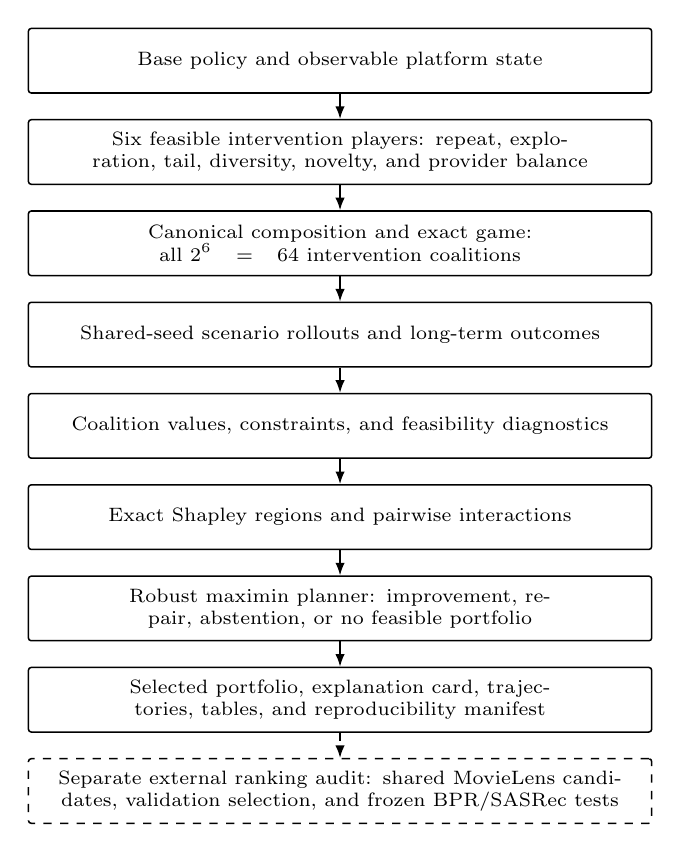
\begin{tikzpicture}[
  font=\scriptsize,
  node distance=3.2mm,
  stage/.style={draw=black, rounded corners=1pt, align=center, text width=0.64\textwidth, minimum height=8.2mm, inner sep=2.2pt, fill=white, line width=.55pt},
  audit/.style={stage, dashed},
  arrow/.style={-{Latex[length=1.6mm]}, draw=black, line width=.6pt}
]
\node[stage] (state) {Base policy and observable platform state};
\node[stage, below=of state] (players) {Six feasible intervention players: repeat, exploration, tail, diversity, novelty, and provider balance};
\node[stage, below=of players] (coalitions) {Canonical composition and exact game: all $2^6=64$ intervention coalitions};
\node[stage, below=of coalitions] (rollouts) {Shared-seed scenario rollouts and long-term outcomes};
\node[stage, below=of rollouts] (values) {Coalition values, constraints, and feasibility diagnostics};
\node[stage, below=of values] (credit) {Exact Shapley regions and pairwise interactions};
\node[stage, below=of credit] (planner) {Robust maximin planner: improvement, repair, abstention, or no feasible portfolio};
\node[stage, below=of planner] (output) {Selected portfolio, explanation card, trajectories, tables, and reproducibility manifest};
\node[audit, below=of output] (external) {Separate external ranking audit: shared MovieLens candidates, validation selection, and frozen BPR/SASRec tests};
\draw[arrow] (state) -- (players);
\draw[arrow] (players) -- (coalitions);
\draw[arrow] (coalitions) -- (rollouts);
\draw[arrow] (rollouts) -- (values);
\draw[arrow] (values) -- (credit);
\draw[arrow] (credit) -- (planner);
\draw[arrow] (planner) -- (output);
\draw[arrow, dashed] (output) -- (external);
\end{tikzpicture}
\caption{Vertical workflow of the proposed \CURE{} framework. The solid path defines, evaluates, attributes, and selects an intervention portfolio. The dashed final box is a separate external ranking audit and is not used to infer causal policy effects from MovieLens.}
\label{fig:workflow}
\end{figure}

\subsection{Exact coalition evaluation and common random numbers}

For a fixed seed and scenario, all coalitions are initialized from the same environment state and use the same event-indexed random-number construction. This common-random-number design aligns stochastic shocks across coalition evaluations and \emph{can} reduce the variance of paired differences when coalition outcomes are positively correlated under shared randomness; an observed difference is then attributable to the policy transformation rather than to a different synthetic cohort draw. Such variance reduction is not guaranteed. Accordingly, we evaluate its effect separately in Section~\ref{sec:reviewer-revision}: in the predeclared stochastic click-feedback variant, the observed variance ratios were approximately one, indicating no material variance reduction in that diagnostic. Seeds are independent across repetitions, and each run writes a manifest, JSONL events, coalition values, attribution regions, interaction regions, decision data, trajectories, and generated tables and figures.

A coalition can still reduce utility, violate relevance, or fail a provider constraint; the grand coalition is in fact harmful in the observed behavioural scenarios. The common-random-number design merely ensures that a comparison between two coalitions is not dominated by an avoidable difference in simulated initial state. We preserve independent seeds because a common-random-number result from one seed is not a stability claim.

Every exact run has three audit layers. The game layer checks that all 64 masks are present for every scenario and that the Shapley efficiency gap is numerically zero. The planner layer records why a coalition is rejected, whether the base is feasible, and whether the final status is improvement, repair, abstention, or no feasible portfolio. The reporting layer materializes numbered tables and figures plus an asset registry. This makes the reported result traceable from a manuscript number to a seed, a configuration hash, and the underlying coalition rows.

The computational cost is transparent. With six players and four behavioural scenarios, one seed requires $64\times4=256$ rollouts. The full behavioural inference study has 20 seeds, or 5,120 scenario--coalition rollouts. The one-at-a-time robustness study evaluates 15 configurations across five seeds; the joint Latin-hypercube study evaluates a baseline plus 24 joint configurations across five seeds. These are substantial but finite computations, and all completed summaries and checksums are retained in the reproducibility snapshot.

\subsection{Attribution, interactions, and direct selection}

The Shapley allocation obeys efficiency within every scenario; since $\Delta\Utility_m(\varnothing)=0$ by definition,
\begin{equation}
 \sum_{i\in\Players}\Shap_i^m=\Delta\Utility_m(\Players).
\label{eq:efficiency}
\end{equation}
This identity is a diagnostic: it is checked to machine precision in every exact game. Pairwise interactions are computed exactly under the declared Grabisch--Roubens convention. Positive interactions identify complementarity, whereas negative interactions identify combinations whose joint effect is lower than their separate effects imply.

Selection does not add Shapley values. Let $\mathcal{F}=\{S\subseteq\Players:\mathbf{1}_{\mathcal F}(S)=1\}$ be the feasible coalitions, with ties broken lexicographically by greater lower improvement, lower cost, smaller cardinality, and smaller canonical mask. The decision rule is casewise:
\begin{equation}
 (S^\star,\mathrm{status})=
 \begin{cases}
 \left(\arg\max_{S\in\mathcal F}\underline\Delta(S),\ \textsc{improvement}\right) & \text{if }\varnothing\in\mathcal F\text{ and }\max_{S\in\mathcal F}\underline\Delta(S)>0,\\[2pt]
 \left(\varnothing,\ \textsc{abstain}\right) & \text{if }\varnothing\in\mathcal F\text{ and }\max_{S\in\mathcal F}\underline\Delta(S)\leq0,\\[2pt]
 \left(\arg\max_{S\in\mathcal F\setminus\{\varnothing\}}\underline\Delta(S),\ \textsc{repair}\right) & \text{if }\varnothing\notin\mathcal F\text{ and }\mathcal F\setminus\{\varnothing\}\neq\emptyset,\\[2pt]
 \left(\varnothing,\ \textsc{no-feasible-portfolio}\right) & \text{if }\varnothing\notin\mathcal F\text{ and }\mathcal F\setminus\{\varnothing\}=\emptyset.
 \end{cases}
\label{eq:improve}
\end{equation}
In improvement mode the base policy is feasible, so abstention is a safe default; in repair mode the base policy violates a constraint and $\varnothing$ is removed from the choice set, so the same maximin criterion chooses the least-worst feasible repair even when its numerical improvement is negative, or certifies that no feasible portfolio exists. This direct objective preserves the meaning of the outcome: Shapley values are explanatory credit; the selected policy is a constrained action.

The explanation card reports both objects. For every selected intervention it records the robust-game Shapley value and the scenario-wise region. For an additional diagnostic it reports the \emph{budget-feasible marginal diagnostic}, defined as the unweighted mean of $\Delta\Utility_m(S\cup\{i\})-\Delta\Utility_m(S)$ over predecessor coalitions for which both $S$ and $S\cup\{i\}$ satisfy the budget constraint. If a player has no budget-feasible predecessor, the diagnostic is undefined and is reported as missing rather than silently set to zero. This quantity is not an axiomatic Shapley value and is not used for selection; it is retained only to expose marginal effects among operationally budget-deployable predecessors. The card header records the selected coalition and its robust lower improvement. This design prevents a familiar but misleading presentation in which a bar chart of attributions is treated as if it were itself an optimization result. A player can have a positive global contribution but not appear in the chosen coalition because it is redundant, consumes scarce injection capacity, violates a constraint in combination, or is dominated by a lower-cost feasible substitute.

The interaction table provides a complementary diagnostic. Let $I_{ij}^m$ denote the declared pairwise interaction of players $i$ and $j$ in scenario $m$. We compute the exact Shapley interaction index
\begin{equation}
 I_{ij}^m=\sum_{S\subseteq\Players\setminus\{i,j\}}
 \frac{|S|!(|\Players|-|S|-2)!}{(|\Players|-1)!}
 \left[\Delta\Utility_m(S\cup\{i,j\})-\Delta\Utility_m(S\cup\{i\})-\Delta\Utility_m(S\cup\{j\})+\Delta\Utility_m(S)\right].
\label{eq:interaction}
\end{equation}
Positive $I_{ij}^m$ means that the joint marginal contribution exceeds the additive baseline under the index; negative interaction means that combining them reduces their expected joint contribution. In the current framework, negative interactions are particularly informative because they often arise from an explicit operational mechanism: slot competition, overlap between long-tail and novelty proposals, or a reranking trade-off. The paper reports interactions as explanatory evidence and does not use a pairwise approximation to replace the exact portfolio search.

\begin{proposition}[Exact credit conservation]\label{prop:efficiency}
For every scenario $m$, the exact allocation in Eq.~\eqref{eq:shapley} satisfies Eq.~\eqref{eq:efficiency}. Thus all credited intervention value equals the full-coalition improvement over the base coalition in that scenario.
\end{proposition}

\begin{proposition}[Coalition well-definedness]\label{prop:well-defined}
Assume that candidate eligibility, score normalization, injection assignment, canonical transformation order, and tie breaking are deterministic conditional on the environment state and random seed. Then every coalition $S\subseteq\Players$ defines one policy transformation $\Policy_S$, independently of the permutation used to compute its Shapley marginal contribution.
\end{proposition}

\begin{proposition}[Repair safety ordering]\label{prop:repair}
If the base coalition is infeasible and $\mathcal{F}$ is nonempty, the repair decision in Eq.~\eqref{eq:improve} selects a feasible coalition whose worst-scenario improvement is no lower than that of any other feasible coalition. It never returns the infeasible base coalition.
\end{proposition}

The propositions do not claim that the finite scenario set is the true real-world environment. They establish properties conditional on the game and constraint definitions, which is the appropriate theoretical level for a decision layer. Proofs are included in Appendix~\ref{app:proofs}.

\subsection{Algorithms and complexity}
\begin{algorithm}[t]
\caption{Exact intervention-game evaluation}\label{alg:game}
\begin{algorithmic}[1]
\Require player set $\Players$; scenario set $\Models$ with scenario parameters $\theta_m$ (fatigue, popularity, satisfaction-shift multipliers); base policy $\BasePolicy$; intervention configuration $\kappa$ (thresholds, capacities, costs $\{c_i\}$); utility parameters $(\gamma,w_s,w_r,w_f,w_c)$; constraint parameters $(B,r_{\min},d_{\max},f_{\max})$; horizon $T$; seed $z$; initial-data specification $D$
\Ensure per-scenario values $\Utility_m(S)$ and $\Delta\Utility_m(S)$; per-scenario constraint margins; exact $\Shap_i^m$ and $I_{ij}^m$; robust game $v^{\mathrm{rob}}$; robust-objective values $\phi_i^{\mathrm{rob}}$; final portfolio decision and diagnostics
\For{each $m\in\Models$}
  \State $X_0\gets$ initialize environment from $D$ under $\theta_m$ and seed $z$; construct event-indexed shocks keyed by $(z,m,t,u,\mathrm{event})$
  \For{each coalition $S\subseteq\Players$ in canonical mask order}
    \State restore the exact copy of $X_0$ (complete simulator state reset)
    \For{$t=0,\ldots,T-1$}
      \State rank with $\BasePolicy$; apply repeat cap, eligibility filtering, the binary injection assignment of Eq.~\eqref{eq:assignment}, diversity, and provider balancing in canonical order
      \State evaluate response and transition with the keyed shocks; record satisfaction, retention, fatigue, relevance, provider exposure, no-ops, collisions, and constraint margins
    \EndFor
    \State store $\Utility_m(S)$ via Eq.~\eqref{eq:utility} with $c(S)$ from Definition~\ref{def:cost}, and store constraint metrics
  \EndFor
  \State compute exact $\phi_i^m$ and $I_{ij}^m$; assert $|\sum_i\phi_i^m-\Delta\Utility_m(\Players)|<\varepsilon_{\mathrm{num}}$
\EndFor
\State compute $v^{\mathrm{rob}}(S)=\min_m\Delta\Utility_m(S)$, feasibility of every $S$, exact $\phi_i^{\mathrm{rob}}$, and the robust decision of Algorithm~\ref{alg:planner}
\end{algorithmic}
\end{algorithm}

\begin{algorithm}[t]
\caption{Improvement/repair portfolio selection. The output distinguishes the decision \emph{mode} (improvement or repair, determined by base feasibility) from the final \emph{status}.}\label{alg:planner}
\begin{algorithmic}[1]
\Require robust lower improvements $\underline\Delta(S)$, feasibility indicators $\mathbf{1}_{\mathcal F}(S)$, coalition costs $c(S)$
\Ensure selected portfolio $S^\star$, mode, and status
\State $\mathcal F\gets\{S\subseteq\Players:\mathbf{1}_{\mathcal F}(S)=1\}$; rank feasible coalitions lexicographically by greater $\underline\Delta(S)$, lower $c(S)$, smaller $|S|$, smaller canonical mask
\If{$\varnothing\in\mathcal F$} \Comment{improvement mode: base policy is constraint-feasible}
  \State $S^\star\gets$ highest-ranked coalition in $\mathcal F$
  \If{$\underline\Delta(S^\star)>0$}
    \State \Return $S^\star$ with mode \textsc{improvement}, status \textsc{improvement}
  \Else
    \State \Return $\varnothing$ with mode \textsc{improvement}, status \textsc{abstention}
  \EndIf
\Else \Comment{repair mode: base policy violates a constraint}
  \If{$\mathcal F\setminus\{\varnothing\}=\emptyset$}
    \State \Return none, with mode \textsc{repair}, status \textsc{no-feasible-portfolio}
  \Else
    \State $S^\star\gets$ highest-ranked coalition in $\mathcal F\setminus\{\varnothing\}$
    \State \Return $S^\star$ with mode \textsc{repair}, status \textsc{repair}
  \EndIf
\EndIf
\end{algorithmic}
\end{algorithm}

For $n=|\Players|$, $M=|\Models|$, and one rollout cost $C_{\mathrm{roll}}$, evaluation costs $O(M2^nC_{\mathrm{roll}})$. The rollout term is not a black box: with horizon $T$, cohort size $|\mathcal{U}|$, catalogue size $|\mathcal{I}|$, slate size $k$, proposal budget $p$ per injection player, and per-item scoring cost $C_{\mathrm{score}}$ of the base ranker, one rollout costs
\begin{equation}
 C_{\mathrm{roll}}=O\!\left(T\,|\mathcal{U}|\left(|\mathcal{I}|\,C_{\mathrm{score}}+|J_S|\,p\log p+\textstyle\prod_{i\in J_S}(1+|C_i|)+k\,C_{\mathrm{rerank}}\right)\right),
\label{eq:croll}
\end{equation}
where the four terms are base ranking, proposal construction and percentile normalization, exact injection assignment, and the bounded greedy diversity/provider reranking passes. Exact Shapley and all pair interactions cost $O(Mn2^n)$ and $O(Mn^2 2^n)$ after coalition values are available. The assignment cost is $O(\prod_{i\in J_S}(1+|C_i|))$; with at most three injection players and top-$10$ proposal lists it remains negligible relative to a rollout. In the full configuration ($M=4$, $n=6$, $T=12$, $|\mathcal{U}|=120$, $|\mathcal{I}|=240$, $k=10$), one seed therefore requires $256$ rollouts; the measured wall-clock time is reported alongside the scalability diagnostics of Section~\ref{sec:reviewer-revision}.

Memory complexity is equally bounded and matters for deployment: the simulator state is $O(|\mathcal{U}|\,|\mathcal{I}|)$ for exposure counts plus $O(|\mathcal{U}|\,d+|\mathcal{I}|\,d)$ for profiles and popularity state; the exact game stores $O(M2^n)$ coalition values and $O(Mn^2)$ interactions; and the run manifest with per-step summaries is $O(T\,M\,2^n)$. No component grows with a training corpus, because coalition evaluation replays rollouts rather than fitting models. The main artifact is deliberately limited to $n=6$; larger libraries require screening or approximate attribution and are evaluated as a separate scalability revision.

\subsection{Controlled oracle regimes}

Before behavioural simulation, nine analytic regimes verify the mechanics of the game and planner: additive, complementary, redundant, antagonistic, short delayed-fatigue, long delayed-fatigue, two provider-repair regimes, and misspecified ambiguity. In well-specified regimes, estimated and oracle games agree by construction. The misspecified regime is intentionally different: the estimated game selects repeat cap while the oracle game selects exploration. It tests whether the framework falsely treats self-consistency as causal recovery. The misspecification diagnostics are: oracle regret, the robust lower improvement lost by deploying the estimated selection instead of the oracle selection; Shapley mean absolute error and sign accuracy between estimated and oracle scenario attributions; and point coverage, the fraction of players whose oracle Shapley value falls inside the estimated scenario Shapley region $[\underline{\Shap}_i,\overline{\Shap}_i]$ of Eq.~\eqref{eq:region}.



\subsection{Behavioural robustness designs}

The behavioural benchmark has four scenarios: nominal, fatigue stress, popularity stress, and mixed stress. The full configuration uses 120 users, 240 items, 18 providers, 10 categories, a 12-step horizon, and a slate of 10. Every numerical scenario parameter---fatigue multipliers $\alpha_m$, popularity-feedback multipliers $\beta_m$, and satisfaction shifts $\delta_m$---is listed in Table~\ref{tab:scenarios} of Appendix~\ref{app:protocol}; nothing about the scenarios is tuned after observing outcomes. The one-at-a-time study changes fatigue strength, repeat threshold, horizon, provider threshold, provider-balance strength, delayed novelty preference drift, and exploration cost. The joint Latin-hypercube study samples these assumptions jointly. Neither study selects a favourable configuration; all configurations and all seed-level decisions are retained. In these designs the environment assumptions vary while the decision-maker's utility weights $(w_s,w_r,w_f,w_c)$ stay fixed; the complementary sensitivity question---varying the objective itself---is studied separately in Section~\ref{sec:objective-sensitivity}.

\begin{figure}[t]
\centering
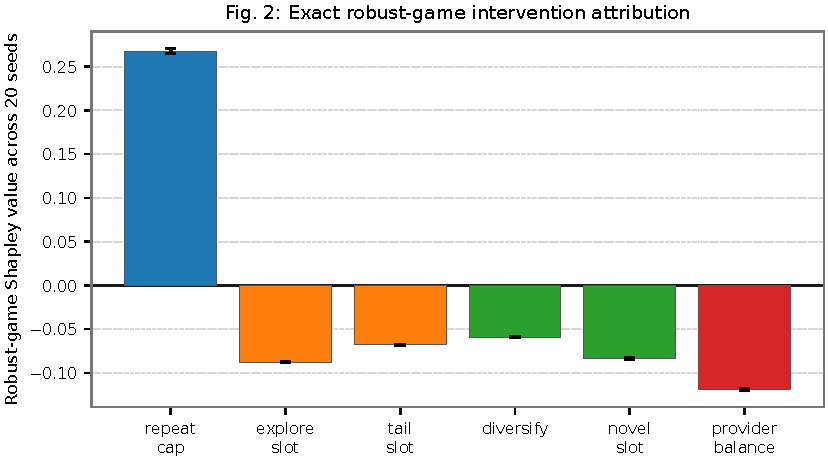
\includegraphics[width=\linewidth]{figures/figure_02_exact_attribution.pdf}
\caption{Exact robust-game Shapley values for the maximin characteristic function across the 20 independent full behavioural seeds. Error bars are seed-level sample standard deviations. This figure is the additive attribution of the actual planner objective, not a scenario-envelope summary.}
\label{fig:lhs}
\end{figure}

\begin{figure}[t]
\centering
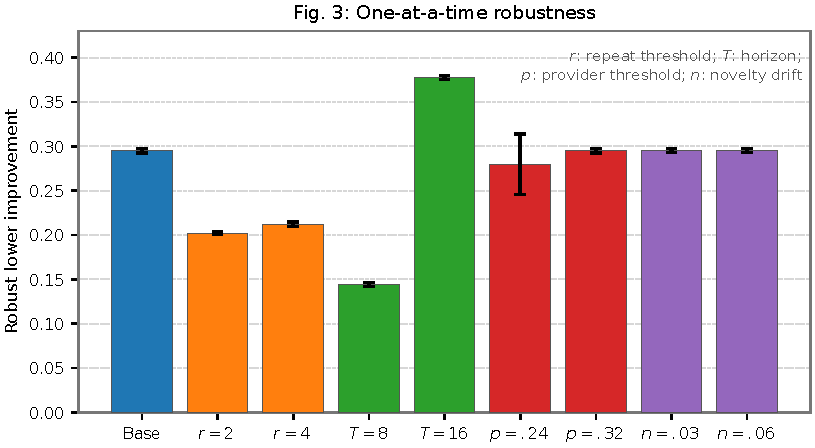
\includegraphics[width=\linewidth]{figures/figure_03_oat_sensitivity.pdf}
\caption{Selected one-at-a-time sensitivity results for mean robust lower improvement: horizon, repeat threshold, provider threshold, and novelty drift are shown; fatigue strength, provider-balance strength, and exploration cost additionally appear in Table~\ref{tab:oat}. Error bars are sample standard deviations over five independent seeds.}
\label{fig:oat}
\end{figure}





\subsection{External ranking protocol}

MovieLens-1M is used only to test recommender implementation robustness. The dataset contains 6,040 users, 3,706 items, and 1,000,209 ratings. A \emph{positive interaction} is a rating of at least four stars ($\mathrm{rating}\geq4$); this threshold is fixed before modelling and yields 575,281 positives. No user-level filtering is applied beyond the split rule below. We construct a chronological leave-one-out split from positive interactions: interactions are sorted per user by timestamp (ties by item identifier), users with fewer than three positives are excluded from evaluation, the last positive of each remaining user is the test target, the previous one is the validation target, and all earlier positives form training. Evaluation then proceeds in ascending user-identifier order over the first 1,000 warm-target users; we report on these 1,000 users, together with one cold test target, rather than silently dropping the cold case or reweighting the evaluation. For every evaluated user, all models receive the identical candidate set
\begin{equation}
 \mathcal{C}_u=\mathcal{I}_{\mathrm{train}}\setminus\mathcal{I}_{u,\mathrm{train}}.
\label{eq:candidates}
\end{equation}
A held-out target absent from the training catalogue is counted as cold rather than silently removed. The final evaluations report 1,000 warm-target users, one cold test target, mean candidate count 3,436.958, and candidate counts from 2,739 to 3,521. For a warm target $i_u^+$ with rank $q_u$ in the ordered candidate list, the per-user metrics are
\begin{equation}
 \mathrm{Recall@}k(u)=\mathbf{1}\{q_u\leq k\},\qquad
 \mathrm{NDCG@}k(u)=\frac{\mathbf{1}\{q_u\leq k\}}{\log_2(q_u+1)},
\label{eq:ranking-metrics}
\end{equation}
and reported values are means over warm evaluated users with cold-target coverage stated separately. Score ties are broken deterministically by ascending item identifier before ranking. Because every evaluated user has exactly one binary held-out target, $\Recall$ coincides identically with Hit Rate at the same $k$; we report the quantity as $\Recall$ in the MovieLens-1M tables and as ``Hit Rate'' in the MovieLens-25M diagnostic, but the two are the same statistic under this protocol. With a single relevant item, $\NDCG$ uses the standard single-target ideal discount. This definition makes the candidate protocol part of the estimand rather than an implementation detail.

The protocol has three gates. First, hyperparameters are selected by validation $\NDCG$ only. Second, the frozen selected configuration is trained once for the final audit and its best validation checkpoint is restored before test ranking. Third, the configuration is replicated over fixed independent seeds without retuning. The evaluator asserts zero seen-item leakage, zero missing-target violations, identical candidates for all compared models, and descending-score correctness. This protocol guards against metric improvements produced by an evaluator difference rather than by a recommender.

The popularity baseline is fit on training interactions only. BPR-MF optimizes the standard Bayesian personalized ranking loss over sampled triples $(u,i,j)$ of a user, a positive item, and a negative item,
\begin{equation}
 \mathcal{L}_{\mathrm{BPR}}=-\frac{1}{|\mathcal{B}|}\sum_{(u,i,j)\in\mathcal{B}}\log\sigma\!\left(x_{ui}-x_{uj}\right),\qquad x_{ui}=e_u^\top e_i+b_i,
\label{eq:bpr-loss}
\end{equation}
with Adam, $L_2$ weight decay, and gradient clipping at norm $5$. Negatives are sampled as an explicit mixture: $30\%$ uniform and $70\%$ popularity-proportional candidates restricted to items the user has not seen in training (a hard-negative branch is also searchable but not selected). SASRec is trained with the same BPR-style loss in which the positive is the next chronological item and the score of a sequence prefix is produced by causal self-attention,
\begin{equation}
 \mathcal{L}_{\mathrm{SASRec}}=-\frac{1}{|\mathcal{B}|}\sum_{(u,i^+,j)\in\mathcal{B}}\log\sigma\!\left(h_u^\top e_{i^+}+b_{i^+}-h_u^\top e_j-b_j\right),
\label{eq:sasrec-loss}
\end{equation}
with AdamW. Both models select hyperparameters by validation $\NDCG$ only, through a predeclared staged search: for BPR, Stage A fixes 64 factors and searches learning rate $\{0.001,0.003,0.01\}$, weight decay $\{10^{-5},10^{-4},10^{-3}\}$, and negative strategy $\{\text{uniform},\text{popularity-mixture},\text{hard-mixture}\}$ (27 configurations, 40-epoch budget each); Stage B refines the top three Stage-A configurations over dimensions $\{32,64,128\}$ and batch sizes $\{2048,4096,8192\}$ (27 configurations); Stage C evaluates popularity-hybrid weights $\alpha\in\{0.25,0.40,0.55,0.70,0.85,1.00\}$ on validation metrics. The selected final BPR configuration uses 128 factors, batch size 8,192, learning rate $0.003$, weight decay $10^{-5}$, and popularity-mixture negatives, trained with a 200-epoch budget and early stopping (patience 15 validation evaluations at every two epochs), restoring the best-validation checkpoint. SASRec is selected independently by validation $\NDCG$ over embedding dimension, sequence length, heads, layers, dropout, batch size, learning rate, weight decay, and negative strategy, using causal self-attention over chronological training prefixes (30-epoch staged budget, 120-epoch final budget with the same early-stopping rule). Its selected configuration has 128-dimensional item embeddings, sequence length 25, two heads, two Transformer layers, dropout 0.10, batch size 1,024, learning rate $5\times10^{-4}$, weight decay $10^{-5}$, and popularity-mixture negatives. The SASRec implementation uses right padding so a causal padding query never encounters an all-masked attention row on the Apple Silicon MPS backend. Both models received the same staged validation budget, and no test metric participates in any selection decision.

The audit also records pairwise training and validation accuracy. These quantities are not used as ranking metrics or selection targets; they are sanity checks that a personalized model has learned a directional preference signal without candidate leakage. For the final SASRec audit, the popularity and SASRec models both have zero critical audit violations and the SASRec best validation epoch equals the restored checkpoint epoch (20). The same audit is rerun within every fixed-configuration replication.

\subsection{Implementation and reproducibility}

The artifact is implemented in Python with typed configuration, deterministic seeds, JSONL events, CSV tables, and a checksumed snapshot. Exact intervention games use CPU-first NumPy simulation. External BPR and SASRec use PyTorch with Apple Silicon MPS when available; BPR uses Adam, item bias, and mixed negatives, while SASRec uses causal self-attention, right-padded sequences, and validation checkpointing. The final snapshot stores source manifests, final configurations, audit tables, loss and validation histories, seed metrics, paired metrics, calibration summaries, controlled-regime assets, and SHA-256 checksums. The code and the manuscript assets are available with the project repository.

\section{Experimental results}\label{sec:results}

\subsection{Research questions and evidence levels}

We answer five questions. \textbf{RQ1}: does the exact game and planner recover known structures and distinguish estimated from oracle recovery? \textbf{RQ2}: which intervention portfolio is selected in the behavioural sequential environment, and how stable is the decision across independent seeds? \textbf{RQ3}: do isolated and joint changes to disclosed behavioural assumptions preserve or alter the decision? \textbf{RQ4}: do audited BPR and SASRec implementations improve chronological ranking over popularity on a real benchmark under the same candidates? \textbf{RQ5}: does the complete \CURE{} decision rule make different and better-held-out decisions than simpler selectors in configurations where they disagree, how sensitive is the decision to the declared utility weights and constraint vector, and does the decision layer remain consistent when the base policy is a learned ranker?

The evidence level differs by question. RQ1--RQ3 and RQ5 make controlled causal-oracle and behavioural claims about \Sim{}. RQ4 makes an external ranking claim on MovieLens-1M and MovieLens-25M. It is not evidence that a MovieLens policy intervention would cause the corresponding long-run platform effect, and it does not validate the portfolio-selection layer.

\subsection{RQ1: controlled recovery and misspecification}\label{sec:rq1}

Table~\ref{tab:regimes} reports the controlled-regime result. The estimated game reproduces the specified estimated selection in all nine regimes. Oracle selection agrees in eight. The exception is deliberately misspecified: the estimated game selects \texttt{repeat\_cap}, while the oracle selects \texttt{explore\_slot}. Estimated recovery is therefore not treated as proof of oracle recovery. The misspecified setting has oracle regret $0.19$, Shapley mean absolute error $0.06$, sign accuracy $0.667$, and point coverage $0.667$.

\begin{table*}[t]
\caption{Controlled oracle-regime validation. ``Estimated match'' compares the selected estimated-game portfolio with the declared estimated target; ``oracle match'' compares it with the true-game portfolio.}\label{tab:regimes}
\centering
\scriptsize
\setlength{\tabcolsep}{3pt}
\resizebox{\textwidth}{!}{%
\begin{tabular}{@{}llccc@{}}
\toprule
Regime & Estimated selected portfolio & Oracle selected portfolio & Estimated match & Oracle match / regret\\
\midrule
Additive & repeat cap + exploration + tail + provider balance & repeat cap + exploration + tail + provider balance & yes & yes / 0.00\\
Complementary & repeat cap + exploration & repeat cap + exploration & yes & yes / 0.00\\
Redundant & tail slot & tail slot & yes & yes / 0.00\\
Antagonistic & exploration slot & exploration slot & yes & yes / 0.00\\
Delayed fatigue, short horizon & abstain & abstain & yes & yes / 0.00\\
Delayed fatigue, long horizon & repeat cap & repeat cap & yes & yes / 0.00\\
Provider repair, balancing & provider balance & provider balance & yes & yes / 0.00\\
Provider repair, repeat & repeat cap & repeat cap & yes & yes / 0.00\\
Misspecified ambiguity & repeat cap & exploration slot & yes & no / 0.19\\
\bottomrule
\end{tabular}}
\end{table*}

This result establishes a needed negative control. A cooperative attribution layer can be internally consistent and still be wrong when its model of the environment is wrong. The paper therefore reports estimated and oracle recovery separately rather than compressing them into one success rate.

The remaining regimes test the distinction between contribution and decision. In the complementary regime, repeat cap and exploration are weak alone but selected jointly. In the redundant regime, tail and novelty overlap and the planner selects one player under its deterministic cost and tie rule. In the antagonistic regime, exploration and diversity are individually useful but jointly harmful, so the selected policy avoids the pair. The two provider-repair regimes start from an infeasible base and select different repairs: provider balancing in one and repeat suppression in the other. These cases show why a framework that independently ranks interventions cannot substitute for a coalition search with explicit repair semantics.

The short- and long-horizon delayed-fatigue regimes additionally test temporal interpretation. With the short horizon, the base is feasible and the planner abstains because repeat suppression has not yet recovered its immediate cost. With the longer horizon, repeat cap is selected. The switch is not a change in implementation or attribution convention; it is a change in the declared decision horizon. This is the minimal controlled demonstration that a myopic metric and a long-horizon intervention decision need not agree.

\subsection{RQ2: behavioural selection over independent seeds}\label{sec:rq2}

The full behavioural study evaluates all 64 coalitions under four scenarios across 20 independent seeds. Repeat cap is selected in 20/20 seeds. The mean robust lower improvement is $0.29371$ with standard deviation $0.00258$, range $[0.28928,0.29709]$, and an approximate $t$-interval of $[0.29250,0.29491]$ (CURE-Sim normalized utility units). Fourteen of 20 decisions are repairs because the base violates the provider-disparity constraint; six are improvements from a feasible base. The selected portfolio is feasible in every seed. Table~\ref{tab:behavioural} summarizes the three seed studies.

The independent five-seed full run provides a second check: repeat cap is selected in 5/5 seeds, with mean lower improvement $0.29488$ and standard deviation $0.00244$. The quick configuration is intentionally not used for inference: it selects repeat cap in four seeds and repeat cap plus tail slot in one, with one negative-improvement repair. It is retained as a smoke and runtime result rather than as an empirical conclusion.

\begin{table}[t]
\caption{Behavioural exact-game seed studies. Lower improvement is the worst-scenario utility change relative to the base policy.}\label{tab:behavioural}
\centering
\scriptsize
\setlength{\tabcolsep}{3pt}
\resizebox{\linewidth}{!}{%
\begin{tabular}{@{}lrrrrl@{}}
\toprule
Study & Seeds & Repeat-cap selection & Lower improvement & SD & Planner modes\\
\midrule
Quick five-seed & 5 & 4/5 & 0.01241 & 0.03908 & 4 improve, 1 repair\\
Full five-seed & 5 & 5/5 & 0.29488 & 0.00244 & 1 improve, 4 repair\\
Full twenty-seed & 20 & 20/20 & 0.29371 & 0.00258 & 6 improve, 14 repair\\
\bottomrule
\end{tabular}}
\end{table}

The grand coalition is budget-infeasible in every seed of the full configuration ($c(\Players)=0.49>B=0.35$), and its raw robust-game value is negative: for example, $\underline{\Delta}(\Players)=-0.14430$ at seed 42 (CURE-Sim normalized utility units), computed directly from the scenario-indexed coalition values. Table~\ref{tab:selector-baselines} reports this raw value separately from the zero fallback payoff of the grand-coalition \emph{selector}, which deploys the full coalition only when it is feasible. The grand coalition is retained only as a diagnostic, not as a selectable portfolio. This rejects an additive ``more interventions is always better'' interpretation. Interaction analysis explains why: several injection and reranking combinations introduce relevance, cost, or fatigue trade-offs that a single-intervention ablation cannot expose.

\begin{table*}[t]
\caption{Held-out selector evaluation. Portfolios are selected on five seeds and evaluated on 20 disjoint seeds. The independent inferential unit is the evaluation seed; 100 cross-product rows are retained for traceability but are not treated as 100 independent observations.}\label{tab:selector-baselines}
\centering
\scriptsize
\setlength{\tabcolsep}{3pt}
\resizebox{\textwidth}{!}{%
\begin{tabular}{@{}lrrrl@{}}
\toprule
Selector & Held-out robust lower improvement & SD & Difference versus CURE & Exact sign-test $p$\\
\midrule
CURE exact maximin & 0.294584 & 0.002031 & --- & ---\\
Best singleton & 0.294584 & 0.002031 & 0.000000 & 1.000000\\
Robust Shapley-1 & 0.294584 & 0.002031 & 0.000000 & 1.000000\\
Robust Shapley-budget & 0.294584 & 0.002031 & 0.000000 & 1.000000\\
Greedy robust & 0.294584 & 0.002031 & 0.000000 & 1.000000\\
Nominal-scenario selector & 0.294584 & 0.002031 & 0.000000 & 1.000000\\
Random feasible & 0.059153 & 0.112314 & -0.235431 & 0.000002\\
Grand-coalition diagnostic\footnotemark[1] & 0.000000 & 0.000000 & -0.294584 & 0.000002\\
\bottomrule
\end{tabular}}
\footnotetext[1]{The grand-coalition row reports the \emph{effective selector payoff after infeasibility handling}: the grand-coalition selector deploys the full coalition when it is feasible and otherwise falls back to the empty coalition, whose improvement is $0$ by definition. The raw robust-game value of the grand coalition is negative in this configuration (Section~\ref{sec:rq2}); it is budget-infeasible in every evaluation seed, so the fallback payoff is what this selector actually delivers. The two quantities are therefore consistent: $0.000000$ is not the raw robust value of the grand coalition.}
\end{table*}

The selector comparison is intentionally not a manufactured superiority claim. Exact CURE, singleton, robust-Shapley, greedy, and nominal selectors all choose repeat cap for all selection seeds in this configuration, so they are tied on the held-out evaluation. The exact framework is markedly better than random feasible selection; the grand coalition is budget-infeasible in every configuration that retains the declared costs and budget ($c(\Players)=0.49>B=0.35$), and is reported only as a diagnostic. The value of CURE-Rec in this regime is therefore not that it beats every heuristic, but that it identifies and explains the same simple intervention while retaining principled repair, constraint, and interaction diagnostics. Because a tied comparison cannot establish the value of the exact decision machinery, we additionally report held-out selector comparisons on configurations in which the selectors genuinely disagree (Section~\ref{sec:divergent-selectors}).

The decision modes are as informative as the selected player. In the full twenty-seed study, the base is infeasible in 14 seeds, principally because provider disparity crosses the declared upper bound. Those 14 outputs are repairs, not failed improvements: repeat cap is chosen because it produces the best feasible maximin policy under the configured scenarios. In the remaining six seeds, the base is feasible and repeat cap is selected as an improvement. A manuscript that reported only the 20/20 selection frequency would hide this operational distinction.

The result also illustrates why the full coalition is not a useful default. A system might reason that enabling all safeguards is conservative. Here, the grand coalition is repeatedly harmful because three slot interventions compete for capacity, rerankers can reduce relevance, and total cost can exceed the budget. Exact enumeration makes this failure visible without assuming pairwise additivity. In a larger intervention library, screening or approximation would be required; the present six-player study provides a clean benchmark in which the portfolio optimum is known exactly.

\subsection{RQ3: calibration robustness and portfolio switches}\label{sec:rq3}

The one-at-a-time study contains 15 predeclared configurations and five seeds per configuration. Repeat cap appears in every selected portfolio (75/75 seed decisions); it is the exact portfolio in 74/75 decisions. The exception occurs at the strict provider threshold 0.24, where one seed selects repeat cap plus tail slot. The result is stable but not invariant in magnitude. Shortening the horizon from 12 to 8 reduces mean lower improvement from $0.29488$ to $0.14397$; extending it to 16 increases it to $0.37785$. Altering the repeat threshold to 2 or 4 changes the mean to $0.20206$ and $0.21226$, respectively. These are expected behavioural sensitivities, not a failure of the framework.

\begin{table*}[t]
\caption{Selected one-at-a-time calibration results. Every row has five independent seeds. The table reports actual archived summaries.}\label{tab:oat}
\centering
\scriptsize
\setlength{\tabcolsep}{3pt}
\resizebox{\textwidth}{!}{%
\begin{tabular}{@{}lrrrll@{}}
\toprule
Assumption & Value & Lower improvement mean & SD & Base-feasible rate & Modal portfolio\\
\midrule
Baseline & --- & 0.29488 & 0.00244 & 0.20 & repeat cap\\
Fatigue strength & 0.75 & 0.29488 & 0.00244 & 0.20 & repeat cap\\
Fatigue strength & 1.25 & 0.29488 & 0.00244 & 0.20 & repeat cap\\
Repeat threshold & 2 & 0.20206 & 0.00175 & 0.20 & repeat cap\\
Repeat threshold & 4 & 0.21226 & 0.00240 & 0.20 & repeat cap\\
Horizon & 8 & 0.14397 & 0.00230 & 0.60 & repeat cap\\
Horizon & 16 & 0.37785 & 0.00220 & 0.20 & repeat cap\\
Provider threshold & 0.24 & 0.27997 & 0.03397 & 0.00 & repeat cap (modal frequency 4/5)\\
Provider threshold & 0.32 & 0.29488 & 0.00244 & 0.60 & repeat cap\\
Provider-balance strength & 0.15 & 0.29488 & 0.00244 & 0.20 & repeat cap\\
Provider-balance strength & 0.55 & 0.29488 & 0.00244 & 0.20 & repeat cap\\
Novelty drift & 0.03 & 0.29502 & 0.00249 & 0.20 & repeat cap\\
Novelty drift & 0.06 & 0.29513 & 0.00252 & 0.20 & repeat cap\\
Exploration cost & 0.05 & 0.29488 & 0.00244 & 0.20 & repeat cap\\
Exploration cost & 0.15 & 0.29488 & 0.00244 & 0.20 & repeat cap\\
\bottomrule
\end{tabular}}
\end{table*}

The Latin-hypercube study is the more stringent test because it changes assumptions jointly. It contains a baseline plus 24 configurations, five seeds each, for 125 decisions. Repeat cap appears in 114/125 selected portfolios, but the framework also selects provider balance, tail-enhanced portfolios, repeat cap plus exploration, and abstention. Across the 25 configuration-level modal portfolios, 18 are repeat cap alone, three are repeat cap plus tail slot, two are provider balance, one is repeat cap plus exploration, and one is abstention. Eighty-three of 125 decisions are repair-mode cases and 42 are improvement-mode cases; four of the improvement-mode cases end in abstention, so mode counts and final-status counts are distinct objects. The result is substantively valuable: the framework does not mechanically choose the same player under joint extreme conditions, yet it produces documented switches tied to feasibility and scenario assumptions.

The LHS study changes the interpretation of the OAT finding. The OAT result supports local robustness: along each isolated axis in the declared range, repeat cap remains present in every selected portfolio. It does not prove global invariance under combined changes. The LHS result supplies the needed qualification. In several joint configurations the modal solution is provider balancing, and in another the modal choice is abstention. These cases are not discarded as inconvenient outliers. They identify the boundary of the repeat-cap conclusion and show that the framework can express a safety- or constraint-driven portfolio switch rather than merely amplifying the strongest average player.

For reporting, we treat the LHS configurations as a predeclared stress design rather than as an iid sample from a real distribution of platforms. The counts $114/125$ and $83/125$ are therefore descriptive frequencies over the design, not estimates of an unknown global deployment probability. This is more precise than calling the design a confidence study while still giving an operator a concrete map of the regions in which the selected policy changes.

\begin{figure}[t]
\centering

\includegraphics[width=0.90\linewidth]{figures/figure_04_attribution_decision.pdf}
\caption{Attribution--decision relationship over the joint calibration design. Each point is one intervention; the horizontal coordinate is its mean Shapley value across the 125 LHS games and the vertical coordinate is its portfolio inclusion rate over the same 125 decisions. The mean aggregates heterogeneous games and can hide sign reversals in individual configurations; it should be read as a design-level summary, not as a per-configuration attribution. Provider balance illustrates why a feasibility-driven portfolio may be selected despite a negative mean unconstrained contribution.}
\label{fig:lhs-stability}
\end{figure}

\subsection{RQ4: external ranking robustness on MovieLens-1M}\label{sec:rq4}

The external evaluation is deliberately separated from the causal benchmark. Popularity, BPR-MF, and SASRec use the same chronological split and candidates. BPR is selected through staged validation search, then audited once and replicated over fixed seeds. SASRec is selected by validation $\NDCG$, audited once on the untouched test set, and replicated without retuning. The final audit has zero seen-item, missing-target, candidate-equality, and descending-score violations for every compared model.

Table~\ref{tab:external} reports the five-seed fixed-configuration summaries. Popularity has $\Recall=0.049$ and $\NDCG=0.02552$. BPR reaches $0.08800\pm0.00354$ recall and $0.04384\pm0.00167$ NDCG. SASRec reaches $0.14520\pm0.00311$ recall and $0.07424\pm0.00281$ NDCG. All SASRec seed-level gains over popularity are positive: recall gains range from $0.091$ to $0.099$ and NDCG gains from $0.04553$ to $0.05293$. These are reproducible ranking results under the protocol; they are not estimates of causal intervention benefit.

At the seed level, the paired differences against popularity are all positive for both models and both metrics (5/5 seeds). The exact two-sided sign test on five paired seeds has a minimum attainable $p$-value of $2(0.5)^5=0.0625$, which is not conventionally significant; a paired $t$-test on the five seed differences is significant ($|t(4)|\geq24.6$, $p\leq1.6\times10^{-5}$, $d_z\geq11.0$) but treats optimizer seeds as the inferential unit and assumes normality of seed effects. We are explicit about what is \emph{not} available: the archived audit stored seed-level aggregates, not per-user outcomes, so user-level paired inference---paired bootstrap confidence intervals, exact McNemar tests on per-user hit indicators, and paired permutation tests on NDCG, with Holm correction across the model$\times$metric family---cannot be computed retroactively from the archive. This analysis is pre-specified for the next audit run in Section~\ref{sec:limitations}; until it is executed, the MovieLens-1M comparison supports stable-improvement language at the seed level but not a user-level significance claim. The MovieLens-25M diagnostic of Section~\ref{sec:reviewer-revision}, in contrast, retained per-user outcomes and reports the full user-level paired analysis (bootstrap confidence intervals, sign-test $p$-values, effect sizes, and Holm adjustment).

\begin{table}[t]
\caption{MovieLens-1M fixed-configuration five-seed ranking results under shared warm-item candidates. Mean $\pm$ sample standard deviation over optimizer seeds; popularity is deterministic for the fixed split. With one binary held-out target per user, $\Recall$ equals Hit Rate.}\label{tab:external}
\centering
\scriptsize
\setlength{\tabcolsep}{2pt}
\resizebox{\linewidth}{!}{%
\begin{tabular}{@{}lrrrr@{}}
\toprule
Model & $\Recall$ & $\NDCG$ & $\Delta\Recall$ vs. popularity & $\Delta\NDCG$ vs. popularity\\
\midrule
Popularity & 0.04900 & 0.02552 & --- & ---\\
BPR-MF + bias & $0.08800\pm0.00354$ & $0.04384\pm0.00167$ & $0.03900\pm0.00354$ & $0.01832\pm0.00167$\\
SASRec & $0.14520\pm0.00311$ & $0.07424\pm0.00281$ & $0.09620\pm0.00311$ & $0.04872\pm0.00281$\\
\bottomrule
\end{tabular}}
\end{table}

\begin{figure}[t]
\centering
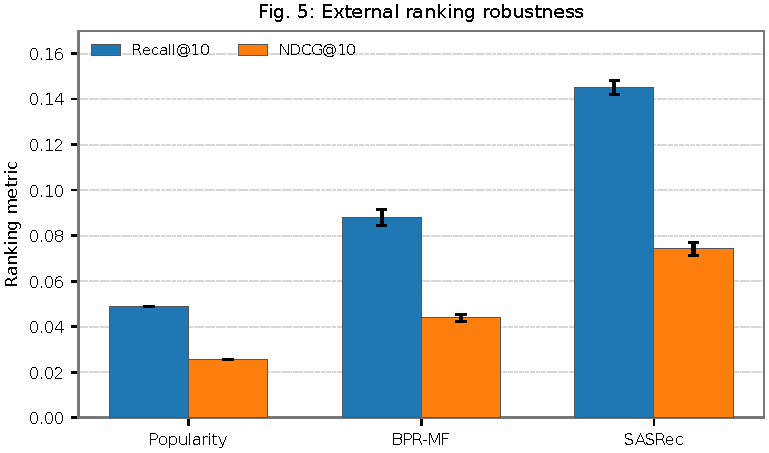
\includegraphics[width=0.94\linewidth]{figures/figure_05_external_ranking.pdf}
\caption{External MovieLens-1M ranking results under the shared warm-item protocol. BPR-MF and SASRec bars show five-seed means with sample-standard-deviation error bars over optimizer seeds; popularity is deterministic for the fixed split. Seed-level error bars quantify optimization stability, not user-level uncertainty; user-level paired confidence intervals are pre-specified for the next audit run (Section~\ref{sec:limitations}) because the archived audit stored seed-level aggregates.}
\label{fig:external}
\end{figure}

\subsection{Ablations, reporting checks, and negative evidence}\label{sec:ablations}

Several checks prevent the reported outcome from becoming a favourable-only story. The controlled misspecification regime fails oracle recovery as intended. The quick behavioural sweep is unstable and is not used for inference. OAT calibration shows that horizon and repeat mechanics materially change utility magnitude. LHS calibration shows that repeat cap is not a universal answer under joint extremes. The external evaluator records one cold target instead of erasing it, and checks the candidate vector used by each model. Finally, the selected SASRec configuration is a pure SASRec configuration rather than a popularity blend chosen after observing test results.

We report seed dispersion rather than treating repeated seeds as independent real-world users. The five external seeds establish optimization stability for a fixed split and candidate protocol, not population-level uncertainty over users, datasets, or deployment contexts. The 20 behavioural seeds establish simulation stability under the declared environment, not a confidence interval for an unspecified production platform.

\subsection{Additional robustness analyses: selection, approximation, CRN, and a second dataset}\label{sec:reviewer-revision}

We conducted several additional robustness analyses without changing the pre-specified primary CURE-Sim configuration. First, a held-out selector experiment used seeds 42--46 for portfolio selection and disjoint seeds 200--219 for evaluation. Because the base policy was infeasible under the full configuration, selection operated in repair mode. The frozen repeat-cap portfolio achieved a robust lower improvement of $0.29235$ and an upper improvement of $0.31500$ on the held-out seeds. This result assesses simulator-conditional generalization across random seeds and should not be interpreted as evidence of real-world causal policy performance.

The maximin-versus-mean and hard-constraint-versus-penalty ablation selected repeat-cap in every tested condition, including penalty coefficients $\{0,0.25,0.5,1,2,5,10\}$. We report this as a null decision ablation: under the pre-specified full configuration, repeat-cap is dominant and scalarization choices do not change the selected mask. It should not be described as evidence that maximin is universally superior. The sampled-attribution study compared budgets 32, 128, 512, and 2048 against exact six-player values. Sign agreement and rank correlation were one at every budget; the MAE decreased from $0.00219$ at budget 32 to $0.00038$ at budget 2048. These are approximation diagnostics, while exact six-player Shapley remains the primary result.

The CRN study used a predeclared stochastic click-feedback variant with click-feedback weight $0.35$, pairs $0\to1$ and $1\to5$, and 20 seeds (300--319). The variance ratios were $1.00122$ and $1.00121$, with bootstrap intervals $[0.99763,1.00601]$ and $[0.97816,1.03538]$, respectively. Thus, common random numbers did not materially reduce paired-difference variance in these tests. This null result is reported as a diagnostic of the declared stochastic simulator variant, not as a CRN benefit.

We also evaluated a distinct 6/8/10-player attribution-approximation benchmark with coalition counts 64, 256, and 1024 and sampled budgets 32--2048. The added players were session-length cap, freshness quota, provider cooldown, and category-coverage quota. In the archived version of this benchmark the additional operators were declared value functions rather than executed policy semantics, so the archived 8/10-player numbers remain an arithmetic scalability stress test rather than a causal CURE-Sim scalability claim. As a revision, all four operators are now implemented as actual slate transformations with disclosed semantics (one-step repeat control via previous-slate demotion; a quota guaranteeing never-exposed, then least-exposed, items; a provider cooldown after concentrated previous-slate exposure; and a category-coverage quota enforced by greedy swaps), and an exact integrated-game driver runs the full rollout-based game for $n=6,8,10$, reporting wall-clock time, peak memory, the Shapley efficiency gap, exact-versus-sampled fidelity, and selection regret. Table~\ref{tab:integrated-scalability} reports the integrated $n=8$ game under the full configuration (seed 42): 256 coalitions $\times$ 4 scenarios complete in 7,505 wall-clock seconds with 114 MB peak memory; the exact Shapley efficiency gap is zero; the planner's decision is unchanged from the six-player game (repeat cap, repair mode, lower improvement $0.298514$), and the selection regret against both the oracle-best and the best feasible frozen mask is exactly $0$. The two integrated operators receive negative robust attributions ($-0.065577$ for session-length cap, $-0.050246$ for freshness quota) and are correctly excluded. Exact-versus-sampled fidelity at $n=8$ degrades gracefully: MAE $0.001290$ at budget 32 and $0.000199$ at budget 2048, with sign agreement and rank correlation equal to one at every budget. The compute-heavy integrated $n=10$ game (1,024 coalitions $\times$ 4 scenarios) is executed through the revision closure notebook (\texttt{notebooks/13\_reviewer\_closure\_runs.ipynb}); outputs are archived under \texttt{integrated\_scalability/players\_10/}.

\begin{table}[t]
\caption{Integrated scalability with real operator semantics (full configuration, seed 42). The $n=6$ rows are the archived primary game; the $n=8$ game integrates session-length cap and freshness quota as executed slate transformations.}\label{tab:integrated-scalability}
\centering
\scriptsize
\setlength{\tabcolsep}{3pt}
\resizebox{\linewidth}{!}{%
\begin{tabular}{@{}lrrrrll@{}}
\toprule
Players & Coalitions & Wall clock (s) & Peak memory (MB) & Efficiency gap & Decision & Selection regret\\
\midrule
$n=6$ (archived) & 64 & 1,804 & $\leq$114 & 0 & repeat cap (repair), $0.298514$ & 0\\
$n=8$ (integrated) & 256 & 7,505 & 114 & 0 & repeat cap (repair), $0.298514$ & 0\\
\bottomrule
\end{tabular}}
\end{table}

Finally, MovieLens-25M was downloaded automatically and evaluated under a separate chronological warm-item protocol. Because this diagnostic retained one hit/NDCG row per evaluated user, it supports the user-level paired analysis that the MovieLens-1M archive does not: for 1,000 paired users, the NumPy BPR fallback was below popularity by $-0.046$ Hit Rate (95\% paired user bootstrap CI $[-0.060,-0.033]$, $d_z=-0.219$) and by $-0.02040$ NDCG (95\% CI $[-0.02688,-0.01437]$, $d_z=-0.203$); exact sign-test p-values were Holm-adjusted across the two metrics ($5.68\times10^{-14}$). This is descriptive ranking evidence for the tested fallback and dataset, not evidence that BPR is generally inferior and not causal policy evidence. The second dataset therefore supplies a robustness check with an unfavorable outcome rather than a selectively favorable replication.

\subsection{Objective sensitivity: utility weights and the constraint frontier}\label{sec:objective-sensitivity}

The environment studies above vary simulator assumptions while holding the decision-maker's objective fixed. The objective itself, however, is normative: the weights $(w_s,w_r,w_f,w_c)$ encode a platform's declared trade-offs, and the constraint vector $(B,r_{\min},d_{\max},f_{\max})$ encodes its operating limits. We therefore stress the decision with respect to both objects. Because the archived seed-42 exact game (revision asset \texttt{divergent\_selector\_holdout/screening/baseline}) stores the step-aggregated satisfaction, retention, fatigue, relevance, disparity, and cost of every coalition and scenario, utility under any weight vector is a linear recombination of stored outcomes and feasibility under any constraint vector is a threshold test on stored margins; both sweeps are exact recombinations of the archived rollouts and introduce no new simulation noise.

\textbf{Utility-weight sensitivity.} Table~\ref{tab:utility-sweep} reports selection under a predeclared grid of 14 weight vectors around the baseline $(0.70,0.30,0.35,1.00)$: halving and doubling each weight individually, three single-component objectives, an equal-stakeholder vector, and a cost-insensitive variant. In 13 of 14 cases the selected portfolio is unchanged (\texttt{repeat\_cap}, repair mode), with robust lower improvements between $0.055347$ (satisfaction-only) and $0.466289$ (fatigue doubled). The single switch occurs when the cost weight is set to zero: the planner then selects repeat cap plus tail slot. The switch is an objective effect rather than a feasibility effect, because the hard budget constraint is enforced identically in every column; removing cost from the objective changes how the planner ranks feasible portfolios. The utility scale itself moves with the weights, as expected, which is why we report the selected portfolio and the mode as the decision-level outcomes.

\begin{table}[t]
\caption{Utility-weight sensitivity on the archived seed-42 exact game (offline recombination; no new rollouts). Lower improvement is in CURE-Sim normalized utility units.}\label{tab:utility-sweep}
\centering
\scriptsize
\setlength{\tabcolsep}{3pt}
\resizebox{\linewidth}{!}{%
\begin{tabular}{@{}lccccrl@{}}
\toprule
Weight vector & $w_s$ & $w_r$ & $w_f$ & $w_c$ & Mode & Selected portfolio (lower improvement)\\
\midrule
Baseline & 0.70 & 0.30 & 0.35 & 1.00 & repair & repeat cap ($0.298514$)\\
Satisfaction $\times\frac12$ / $\times2$ & 0.35 / 1.40 & 0.30 & 0.35 & 1.00 & repair & repeat cap ($0.261478$ / $0.372267$)\\
Retention $\times\frac12$ / $\times2$ & 0.70 & 0.15 / 0.60 & 0.35 & 1.00 & repair & repeat cap ($0.245180$ / $0.405028$)\\
Fatigue $\times\frac12$ / $\times2$ & 0.70 & 0.30 & 0.175 / 0.70 & 1.00 & repair & repeat cap ($0.214385$ / $0.466289$)\\
Cost $\times\frac12$ / $\times2$ & 0.70 & 0.30 & 0.35 & 0.50 / 2.00 & repair & repeat cap ($0.323514$ / $0.248514$)\\
Satisfaction only & 1.00 & 0.00 & 0.00 & 1.00 & repair & repeat cap ($0.055347$)\\
Retention only & 0.00 & 1.00 & 0.00 & 1.00 & repair & repeat cap ($0.305012$)\\
Fatigue aversion only & 0.00 & 0.00 & 1.00 & 1.00 & repair & repeat cap ($0.429357$)\\
Equal stakeholder & 0.45 & 0.45 & 0.45 & 1.00 & repair & repeat cap ($0.373329$)\\
Cost insensitive & 0.70 & 0.30 & 0.35 & 0.00 & repair & repeat cap + tail slot ($0.353623$)\\
\bottomrule
\end{tabular}}
\end{table}

\textbf{Constraint frontier.} Table~\ref{tab:frontier} reports the planner's mode and portfolio over the full grid $B\in\{0.15,0.25,0.35,0.45,0.55\}$, $r_{\min}\in\{-0.02,-0.08,-0.15\}$, $d_{\max}\in\{0.22,0.28,0.34\}$, and $f_{\max}\in\{0.55,0.65,0.75\}$ (135 combinations), again recomputed offline from the archived margins. The frontier realizes all three non-degenerate decision statuses: 90 repair selections, 30 improvement selections, and 15 abstentions; no combination yields ``no feasible portfolio''. The base policy is feasible in 45 of 135 combinations, and which constraint binds is legible from the grid: the base becomes feasible exactly when the disparity cap is relaxed to $0.34$, identifying provider disparity as the driver of repair mode in this configuration; once the base is feasible, the relevance floor determines abstention-versus-improvement (abstention at $r_{\min}=-0.02$, improvement at the two looser floors), independent of the fatigue cap in this design. The selected portfolio also moves along the frontier (repeat cap, repeat cap plus tail, provider balance, and exploration plus tail portfolios each appear), demonstrating that the improvement/repair/abstention semantics are active properties of the constraint surface rather than fixed labels. Notably, even where the relaxed budget ($B=0.55$) and relevance floor ($r_{\min}\leq-0.08$) render the grand coalition feasible, the planner never selects it: its robust value remains dominated by cheaper portfolios. This confirms that the grand coalition's exclusion at the primary configuration is not an artifact of the budget alone.

\begin{table}[t]
\caption{Constraint-frontier phase diagram over 135 predeclared combinations (offline recombination of the archived seed-42 margins). The left panel counts decision status; the right panel counts the selected portfolio. Both are marginal distributions over the same 135 grid cells and are not paired row-wise.}\label{tab:frontier}
\centering
\scriptsize
\setlength{\tabcolsep}{4pt}
\begin{tabular}{@{}lr@{\hspace{2.5em}}lr@{}}
\toprule
\multicolumn{2}{@{}c}{Decision status (cells)} & \multicolumn{2}{c}{Selected portfolio (cells)}\\
\midrule
Repair selected & 90 & repeat cap & 60\\
Improvement selected & 30 & repeat cap + tail slot & 30\\
Abstain (keep base) & 15 & provider balance & 18\\
No feasible portfolio & 0 & exploration + tail slot & 12\\
 & & abstention & 15\\
\bottomrule
\end{tabular}
\end{table}

The two sweeps have a clear limitation: they condition on a single archived environment seed (seed 42) and on the disclosed simulator mechanisms. They answer the objective-robustness question---whether the declared decision changes when the declared objective or constraints change---and are not evidence about unrepresented environments.

\subsection{Held-out selector comparison where selectors disagree}\label{sec:divergent-selectors}

The archived full-configuration selector study (Table~\ref{tab:selector-baselines}) cannot distinguish the exact planner from simpler selectors, because all substantive selectors select the same portfolio there. To make the comparison nontrivial we predeclared a screening rule: among the archived LHS design points whose five-seed decisions were not always repeat-cap (plus the baseline), screen each configuration with seed 42 and promote the first configuration, in design order, for which at least two of the six substantive selectors choose different masks. The screening order and rule were fixed before inspecting any screening outcome.

The baseline configuration reproduces the known tie: all six substantive selectors select repeat cap. The first divergent configuration in design order is LHS point \texttt{lhs-012} (joint assumptions: fatigue strength $1.390$, repeat threshold $5$, horizon $4$, provider threshold $0.2246$, provider-balance strength $0.6133$, novelty benefit $0.0390$, exploration cost $0.1710$). There the base policy is constraint-infeasible, so the decision operates in repair mode. Table~\ref{tab:divergent-screening} reports the selectors' choices.

\begin{table}[t]
\caption{Selector screening on the divergent configuration \texttt{lhs-012} (seed 42). Repair mode: the base policy is constraint-infeasible, so a valid decision must deploy a non-empty feasible portfolio.}\label{tab:divergent-screening}
\centering
\scriptsize
\setlength{\tabcolsep}{4pt}
\begin{tabular}{@{}llc@{}}
\toprule
Selector & Selected portfolio & Feasible\\
\midrule
CURE exact maximin & provider balance & yes\\
Best singleton & provider balance & yes\\
Robust Shapley-1 & provider balance & yes\\
Nominal-scenario selector & provider balance & yes\\
Robust Shapley-budget & (none; keeps the infeasible base) & no\\
Greedy robust & (none; keeps the infeasible base) & no\\
\bottomrule
\end{tabular}
\end{table}

The divergence is substantive rather than cosmetic. The exact planner, the best-singleton rule, the robust-Shapley-1 rule, and the nominal-scenario selector all identify provider balancing as the best feasible repair, while the budgeted-Shapley-prefix and greedy heuristics terminate at the empty coalition---which, in repair mode, means retaining the constraint-infeasible base policy. This is precisely the failure mode that improvement/repair semantics are designed to prevent: heuristics that compare marginal gains against the base cannot represent the obligation to repair an infeasible base when every repair has a negative unconstrained improvement.

The predeclared held-out protocol then freezes every selector's choice on each of the five selection seeds (42--46) and evaluates all frozen portfolios on the disjoint seeds 200--219. The selection seeds themselves vary in this configuration: the exact planner selects provider balance three times, tail slot once, and abstains once (seed 43, where the base policy is feasible and no portfolio has positive robust improvement); the best-singleton and robust-Shapley-1 rules agree with the planner on four seeds but deploy repeat cap on the abstention seed; the nominal-scenario selector agrees with the planner on all five seeds; and the budgeted-Shapley and greedy rules return the empty coalition on all five seeds. Table~\ref{tab:divergent-holdout} reports the held-out evaluation.

\begin{table*}[t]
\caption{Held-out selector evaluation on the divergent configuration \texttt{lhs-012}. Portfolios are selected on seeds 42--46 and evaluated on disjoint seeds 200--219; the independent inferential unit is the evaluation seed ($n=20$), and the 100 cross-product rows are retained for traceability. Lower improvement is in CURE-Sim normalized utility units; in repair mode it can be negative because the comparison is against an infeasible base policy.}\label{tab:divergent-holdout}
\centering
\scriptsize
\setlength{\tabcolsep}{3pt}
\resizebox{\textwidth}{!}{%
\begin{tabular}{@{}lrrrrl@{}}
\toprule
Selector & Held-out lower improvement & SD & Held-out feasible rate & Paired difference vs.\ CURE & Exact sign-test $p$\\
\midrule
CURE exact maximin & $-0.089270$ & 0.047203 & 0.70 & --- & ---\\
Best singleton & $-0.100579$ & 0.026558 & 0.70 & $-0.011309$ & 0.000002\\
Robust Shapley-1 & $-0.100579$ & 0.026558 & 0.70 & $-0.011309$ & 0.000002\\
Nominal-scenario selector & $-0.089270$ & 0.047203 & 0.70 & 0.000000 & 1.000000\\
Robust Shapley-budget\footnotemark[1] & 0.000000 & 0.000000 & 0.10 & $+0.089270$ & 0.000002\\
Greedy robust\footnotemark[1] & 0.000000 & 0.000000 & 0.10 & $+0.089270$ & 0.000002\\
Random feasible & $-0.263322$ & 0.063987 & 0.75 & $-0.174052$ & 0.000002\\
Grand-coalition diagnostic\footnotemark[1] & 0.000000 & 0.000000 & 0.10 & $+0.089270$ & 0.000002\\
\bottomrule
\end{tabular}}
\footnotetext[1]{These selectors freeze the empty coalition, whose improvement is $0$ by definition. Their numerical payoff is therefore higher than any repair's in every evaluation seed (hence the significant sign test), but the portfolio is constraint-feasible on only 2 of 20 evaluation seeds---exactly the seeds on which the base policy itself is feasible; on the remaining 18 seeds it retains a constraint-violating base policy and is not an admissible decision in repair mode. The sign-test $p$-values compare numerical payoffs only and must be read together with the feasibility rate.}
\end{table*}

Three conclusions follow. First, among selectors that always return a constraint-feasible portfolio, the exact planner achieves the best held-out robust value: it improves on the best-singleton and robust-Shapley-1 rules in 20 of 20 evaluation seeds (paired mean margin $0.011309$, exact sign-test $p=1.9\times10^{-6}$), and it ties the nominal-scenario selector because both freeze identical portfolios. Second, the abstention case is quantified: on the selection seed where the base is feasible, the singleton heuristic deploys repeat cap, whose held-out robust value is negative in all 20 evaluation seeds (mean $-0.056547$), while the exact planner abstains. Third, the comparison exposes what a numerical-payoff comparison alone would hide: the budgeted-Shapley and greedy rules show a positive paired difference ($+0.089270$) against the planner, yet their frozen decision is infeasible in 18 of 20 evaluation seeds. The exact framework's advantage in this configuration is therefore a \emph{decision-validity} advantage---repair semantics and constraint enforcement---together with a modest but consistent robust-value advantage over the feasible heuristic selectors.

We also report the limitation visible in the table without embellishment: the held-out repair selected on the calibration seeds satisfies the declared constraints in 14 of 20 evaluation seeds (feasibility rate $0.70$). Feasibility thus generalizes imperfectly across seeds in this stress configuration, which is consistent with the strict provider-threshold caveat reported earlier and is another reason the planner retains per-seed constraint diagnostics rather than a single point decision.

The second divergent configuration in the declared screening order is LHS point \texttt{lhs-009} (joint assumptions: fatigue strength $1.0941$, repeat threshold $3$, horizon $11$, provider threshold $0.2134$, provider-balance strength $0.3486$, novelty benefit $0.0189$, exploration cost $0.1889$). There the base policy violates the provider-disparity cap ($0.3204>0.2134$), so the decision again operates in repair mode, but the divergence takes a different form (Table~\ref{tab:divergent-screening-2}, seed 42). The exact planner selects the two-intervention portfolio repeat cap plus tail slot with robust lower improvement $+0.192848$, which satisfies all four constraints (disparity $0.1872$). The higher-value portfolio repeat cap alone ($+0.268322$) is disparity-infeasible ($0.2302>0.2134$) and is therefore unavailable; the only feasible singleton is provider balance, whose robust value is \emph{negative} ($-0.118509$), and both the best-singleton and robust-Shapley-1 rules select it. The budgeted-Shapley and greedy rules again return the empty coalition, retaining the constraint-violating base.

\begin{table}[t]
\caption{Selector screening on the divergent configuration \texttt{lhs-009} (seed 42). Repair mode: the base policy is disparity-infeasible.}\label{tab:divergent-screening-2}
\centering
\scriptsize
\setlength{\tabcolsep}{4pt}
\begin{tabular}{@{}llcc@{}}
\toprule
Selector & Selected portfolio & Robust value & Feasible\\
\midrule
CURE exact maximin & repeat cap + tail slot & $+0.192848$ & yes\\
Best singleton & provider balance & $-0.118509$ & yes\\
Robust Shapley-1 & provider balance & $-0.118509$ & yes\\
Nominal-scenario selector & repeat cap + tail slot & $+0.192848$ & yes\\
Robust Shapley-budget & (none; keeps infeasible base) & $0.000000$ & no\\
Greedy robust & (none; keeps infeasible base) & $0.000000$ & no\\
\bottomrule
\end{tabular}
\end{table}

This configuration illustrates two methodological points at once. First, a positive attribution does not identify a good decision: robust-Shapley-1 ranks provider balance as the strongest individual attribution, yet deploying the best singleton loses utility relative to the base. Second, the portfolio optimum lies outside the reach of singleton search even though it has strictly positive value: the best repair requires a coalition, and the best single intervention is itself constraint-infeasible. Only the exact constrained search recovers it.

The held-out protocol on this configuration is summarized in Table~\ref{tab:divergent-holdout-2}. The exact planner's frozen portfolios are positive-valued on every selection seed and always contain repeat cap, paired with a seed-dependent partner (tail slot twice, diversity once, provider balance once); the nominal-scenario selector freezes identical portfolios. The best-singleton and robust-Shapley-1 rules freeze provider balance on four seeds (its screening value is negative) and repeat cap on one; the budgeted-Shapley and greedy rules freeze the empty coalition on four seeds and repeat cap on one.

\begin{table*}[t]
\caption{Held-out selector evaluation on the divergent configuration \texttt{lhs-009}. Portfolios are selected on seeds 42--46 and evaluated on disjoint seeds 200--219; the independent inferential unit is the evaluation seed ($n=20$), and the 100 cross-product rows are retained for traceability. Feasibility rates are computed over the 100 frozen evaluations. Lower improvement is in CURE-Sim normalized utility units.}\label{tab:divergent-holdout-2}
\centering
\scriptsize
\setlength{\tabcolsep}{3pt}
\resizebox{\textwidth}{!}{%
\begin{tabular}{@{}lrrrrl@{}}
\toprule
Selector & Held-out lower improvement & SD & Held-out feasible rate & Paired difference vs.\ CURE & Exact sign-test $p$\\
\midrule
CURE exact maximin & $+0.198583$ & 0.038810 & 0.47 & --- & ---\\
Best singleton & $-0.039305$ & 0.152617 & 0.82 & $-0.237888$ & 0.000002\\
Robust Shapley-1 & $-0.039305$ & 0.152617 & 0.82 & $-0.237888$ & 0.000002\\
Nominal-scenario selector & $+0.198583$ & 0.038810 & 0.47 & 0.000000 & 1.000000\\
Robust Shapley-budget\footnotemark[1] & $+0.052876$ & 0.106289 & 0.02 & $-0.145707$ & 0.000002\\
Greedy robust\footnotemark[1] & $+0.052876$ & 0.106289 & 0.02 & $-0.145707$ & 0.000002\\
Random feasible & $-0.094093$ & 0.167773 & 0.93 & $-0.292677$ & 0.000002\\
Grand-coalition diagnostic & 0.000000 & 0.000000 & 0.00 & $-0.198583$ & 0.000002\\
\bottomrule
\end{tabular}}
\footnotetext[1]{These selectors freeze the empty coalition on four of five selection seeds (repeat cap on the remaining seed). Their frozen portfolios are constraint-feasible in only 2 of the 100 held-out evaluations; in repair mode, freezing the empty coalition means retaining the disparity-infeasible base policy.}
\end{table*}

The held-out comparison is unambiguous in this configuration: the exact planner's frozen portfolios achieve a higher robust lower improvement than every other selector in all 20 evaluation seeds (paired margins $0.145707$ to $0.292677$, exact sign-test $p=1.9\times10^{-6}$ in every comparison), while the singleton-based rules deploy portfolios with \emph{negative} mean held-out value even though a positive multi-intervention repair exists. The price of the strict provider threshold is visible in the feasibility column: the planner's frozen portfolios satisfy the declared constraints in 47 of 100 held-out evaluations, and the base policy itself is infeasible in all 20 evaluation seeds. We report this as the honest generalization behaviour of a stress configuration rather than a failure of the protocol: the planner's per-seed constraint diagnostics are precisely what make the 53 infeasible cases inspectable instead of silent.

\subsection{Semi-real integration: a learned base policy inside the intervention game}\label{sec:semireal}

The primary game is evaluated over a transparent hand-crafted base policy, while the MovieLens audit evaluates learned rankers separately; the reviewer correctly asks where the two evidence paths meet. We bridge them in a disclosed, simulator-conditional way. Under the full configuration and seed 42, we first roll out the default base policy with interaction logging enabled, producing $14{,}400$ impressions with click rate $0.5459$; we then fit a BPR-MF ranker (32 factors, 60{,}000 updates) on that logged feedback, deploy the trained ranker as the base policy, and re-run the exact intervention game on top of it through a policy-factory hook; the coalition semantics, scenarios, constraints, and seeds are unchanged.

\begin{table}[t]
\caption{Semi-real integration (seed 42, full configuration): the exact intervention game evaluated over the hand-crafted base policy versus a BPR-MF ranker trained on simulator-logged feedback. Both decisions operate in repair mode; lower/upper improvements are in CURE-Sim normalized utility units.}\label{tab:semireal}
\centering
\scriptsize
\setlength{\tabcolsep}{3pt}
\resizebox{\linewidth}{!}{%
\begin{tabular}{@{}lllrrrr@{}}
\toprule
Base policy & Mode & Selected & Lower & Upper & Disparity upper & Relevance $\Delta$\\
\midrule
Hand-crafted (history-aware) & repair & repeat cap & 0.298514 & 0.313069 & 0.225872 & $-0.044137$\\
Learned BPR (logged feedback) & repair & repeat cap & 0.335378 & 0.369736 & 0.181806 & $-0.050223$\\
\bottomrule
\end{tabular}}
\end{table}

The decision layer behaves consistently across the two base policies: both games are repair-mode, both select repeat cap, and the robust-objective attributions agree in sign and nearly in magnitude for all six players (repeat cap $+0.274$ vs.\ $+0.317$; the remaining five players negative in both games, e.g.\ provider balance $-0.119$ in both). The learned-base game yields a higher robust lower improvement ($0.335378$ vs.\ $0.298514$) and a lower provider-disparity upper ($0.1818$ vs.\ $0.2259$), while the grand coalition remains harmful under both base policies ($-0.109812$ vs.\ $-0.144299$). The scope of this result is explicit: the feedback loop is still the disclosed \Sim{} mechanism, so this is evidence that the \CURE{} layer is robust to replacing the hand-crafted ranker with a learned one, not evidence about real deployment logs. Integrating a ranker trained on external data inside the simulator requires mapping the external item space into the sequential environment and remains future work (Section~\ref{sec:limitations}).

Taken together, the two divergent configurations answer the question that the tied full-configuration comparison (Table~\ref{tab:selector-baselines}) could not. Where selectors disagree, the exact constrained planner (i) achieves the best held-out robust value in both configurations---among selectors that always return constraint-feasible portfolios in \texttt{lhs-012}, and against every compared selector in \texttt{lhs-009}, in each case in 20 of 20 held-out evaluation seeds; and (ii) finds a positive-valued multi-intervention repair that singleton search cannot reach and that the attribution-ranked singleton rule does not choose (\texttt{lhs-009}). The comparison also quantifies what the simpler rules do when they lack repair semantics: they retain a constraint-violating base policy in 18 of 20 held-out seeds (\texttt{lhs-012}) and freeze the infeasible empty coalition on four of five selection seeds (\texttt{lhs-009}). We stress that these are simulator-conditional decision results under disclosed mechanisms; they establish the value of the decision machinery inside \Sim{}, not real-world policy effectiveness.

\section{Discussion and broader implications}\label{sec:discussion}

\subsection{What the framework explains}

\CURE{} explains a portfolio-level operational decision. A system owner can ask whether repeat suppression is robustly useful, whether provider balancing is required to repair a constraint, whether additional exploration is complementary or redundant, and whether the available evidence supports change at all. The answer is not a feature-level saliency map; it is a coalition value table, an attribution region, an interaction structure, and a decision card. This is useful precisely because recommendation interventions often have consequences outside immediate relevance.

The OAT and LHS results illustrate the difference between robustness and invariance. The OAT result says that repeat cap survives each isolated perturbation in the declared range. The LHS result says that joint changes can move the decision to provider balancing, tail support, a composite intervention, or abstention. A framework that returned repeat cap everywhere would be less credible, not more credible. The observed switches are evidence that constraints and scenario dynamics are participating in the decision.

\subsection{Relationship between causal-oracle and external evidence}

The two evaluation paths answer different questions. \Sim{} supports causal statements internal to a disclosed sequential structural model: the true policy value is known, counterfactual rollouts are executable, and oracle recovery can be measured. MovieLens-1M supports a distinct statement: under a shared chronological ranking protocol, the tested implementations produce stable ranking improvements. It does not record a complete policy assignment mechanism, exposure propensities, or all items made available to users. Consequently, the paper does not translate a MovieLens NDCG improvement into a claimed causal benefit of an intervention portfolio.

This boundary should improve, rather than weaken, the paper. It prevents a common but invalid move from retrospective ratings to long-term policy claims. A future audited production log with slates, propensities, policy identifiers, eligibility, and delayed outcomes could connect the two paths using off-policy or randomized-policy evaluation. The present artifact makes the data requirements visible.

\subsection{Implications for system design}

The results suggest three practical principles. First, interventions should be managed as portfolios, not independent checkboxes. Second, a provider or fatigue constraint changes the meaning of a decision: an intervention can be selected as a repair even when a purely unconstrained comparison would favour keeping the base. Third, attribution should be paired with a decision rule. Ranking interventions by Shapley value alone does not enforce relevance, fatigue, provider, or budget requirements.

The external results add an implementation lesson. On MovieLens-1M specifically, the same candidate protocol and audit exposed large, stable gains from a sequential model over popularity and BPR; the MovieLens-25M diagnostic shows that such ranker-level findings do not necessarily transfer across datasets, since the tested NumPy BPR fallback fell below popularity there. This does not settle which base model a deployment should use, but it demonstrates that \CURE{} can be evaluated beside modern ranking models without changing the meaning of candidates, test targets, or checkpoint selection.

\subsection{Limitations and threats to validity}\label{sec:limitations}

We organize the threats to validity by validity type rather than by experiment.

\textbf{Construct validity.} The scenario set is disclosed but finite; its Shapley regions are sensitivity summaries over the implemented mechanisms, not universal uncertainty intervals. Several decision-critical quantities are normative design choices rather than empirically estimated quantities: the utility weights $(w_s,w_r,w_f,w_c)$ encode a platform's value trade-offs, the intervention costs are synthetic intervention-cost units, and the retention construction couples satisfaction and fatigue by design. The provider-disparity threshold $d_{\max}=0.28$ and the Gini coefficient itself are one particular fairness operationalization among many; equalized provider exposure measured by Gini is not automatically equivalent to fair treatment, since provider eligibility, quality, supply, and contractual context may matter. Similarly, the simulator's fatigue dynamics are a disclosed abstraction and are not validated against observed longitudinal user behaviour. The term ``safe'' used for base policies throughout the paper should be read as ``constraint-feasible under the declared thresholds'', and ``unsafe'' as ``constraint-infeasible''; no normative safety claim is intended or established.

\textbf{Internal validity.} The behavioural environment abstracts from many deployment phenomena, including strategic providers, dynamic inventory, policy learning, and heterogeneous user objectives. Event ordering is fixed by the canonical composition and the keyed shock stream, so coalition semantics are deterministic within a seed; nevertheless, an alternative cohort-update ordering could quantitatively change the popularity and fatigue trajectories, and such ordering choices are part of the disclosed simulator rather than identified facts. The intervention library is deliberately small and does not include model retraining, UI changes, or arbitrary causal graph discovery. Exact enumeration scales exponentially with the number of players, so the current design is appropriate for a bounded operational library rather than hundreds of interventions.

\textbf{External validity.} The calibration studies are designed robustness probes, not empirical calibration to MovieLens. The LHS configurations are predeclared and retained, but a finite design cannot cover every combination of environment assumptions. The MovieLens evaluation is limited to one benchmark family, one chronological split per dataset, 1,000 evaluated warm-target users, and five optimization seeds; its shared candidates improve comparability while making the metric a warm-item ranking metric by design, and cold targets are counted but not ranked. Critically, the external BPR and SASRec models are evaluated as rankers, whereas the causal game is evaluated inside \Sim{}: the real ranking evaluation is separate from the \CURE{} intervention mechanism. The semi-real experiment of Section~\ref{sec:semireal} narrows this gap by deploying a learned ranker as the simulator base policy, but the feedback loop remains the disclosed simulator mechanism; no result in this paper validates \CURE{} portfolio selection on real intervention data. Establishing that effectiveness requires audited real policy logs or randomized policy experiments, which remains future work.

\textbf{Statistical conclusion validity.} The 20 behavioural seeds support simulator-conditional stability statements, not population-level confidence intervals over platforms. The five external seeds are optimization replicates of one split; with $n=5$ paired seeds the exact sign test cannot reach conventional significance, and the archived MovieLens-1M audit retained seed-level aggregates rather than per-user outcomes. We do not report a formal power analysis: the seed budgets follow the predeclared audit protocol rather than a target effect size, which is itself a limitation---small seed budgets cannot certify the absence of effects. We therefore pre-specify the user-level analysis for the next audit run: export one hit/NDCG row per evaluated user and per frozen seed, compute paired bootstrap confidence intervals for mean differences, exact McNemar tests on hit indicators, paired permutation tests for NDCG, Cohen $d_z$ effect sizes, and Holm correction across the model$\times$metric family, together with a power consideration for the user-level tests. Until that run is executed and archived, MovieLens-1M conclusions are restricted to seed-level stability under the audited protocol.

\textbf{Responsible AI statement.} The framework is designed to make normative choices inspectable rather than to settle them: utility weights, costs, and constraint thresholds are declared inputs, every rejected portfolio is logged with its violated constraints, and the planner reports abstention or the absence of any feasible portfolio instead of forcing an intervention. Provider-disparity and fatigue constraints should be set through platform policy, regulation, or stakeholder consultation rather than inferred from the simulator; the threshold values used here are disclosed configuration choices, not empirical standards. The MovieLens experiments use public benchmark data under their terms of use and involve no human subjects.

\subsection{Reproducibility and reporting checklist}

The final result snapshot contains 52 SHA-256 entries covering the implementation manifests and the small final artifacts needed to reproduce the reported numbers. Raw MovieLens data and large training checkpoints are not duplicated in the archive; this avoids redistribution of source data and unnecessary storage while retaining configuration hashes, selected hyperparameters, validation histories, final audit tables, and fixed-seed metrics. A reader can verify the snapshot with \texttt{sha256sum -c SHA256SUMS.txt} before inspecting the tables.

For a claim paper, reproducibility also requires negative evidence. The archive therefore includes the misspecified controlled regime, the quick sweep that is not used for inference, all OAT and LHS configuration summaries, seed-level rather than only mean metrics, and constraint-mode fields. The paper does not hide that the external data path is evidentially weaker for causal questions than the oracle path. This reporting design is intended to make it possible to disagree with the scope of the claim without being unable to inspect the computation.

\section{Conclusion}\label{sec:conclusion}

\CURE{} formulates a bounded set of recommendation-policy transformations as an exact cooperative decision problem combining scenario-indexed coalition values, Shapley attribution, interaction analysis, hard feasibility constraints, and robust portfolio selection. Controlled regimes establish the intended behaviour of the framework under additive, complementary, redundant, antagonistic, delayed, repair, and misspecified settings, while behavioural stress tests show both local stability and portfolio switching under joint parameter changes. The separate MovieLens-1M experiment demonstrates stable ranking gains for the tested BPR-MF and SASRec implementations under a common warm-item evaluation protocol, whereas the additional MovieLens-25M experiment illustrates that such ranker-level findings do not necessarily transfer across datasets. These external ranking experiments validate the shared evaluation pipeline and the implemented rankers; they do not establish the causal value of \CURE{} interventions.

The principal contribution is a disciplined bridge from intervention attribution to action. It is not enough to assign a large credit value to an intervention; a platform needs to know whether a feasible portfolio robustly improves a constraint-feasible base policy or repairs a constraint-infeasible one. By keeping causal-oracle claims, behavioural robustness claims, and external ranking claims separate, the artifact provides a reproducible foundation for future evaluation with audited production policy logs. The effectiveness of \CURE{} for selecting interventions in audited real policy logs remains to be established.

\backmatter

\bmhead{Supplementary information}
The reproducibility snapshot contains checksumed configurations, exact-game summaries, controlled-regime assets, OAT and LHS calibration summaries, BPR and SASRec audit outputs, loss histories, validation histories, seed-level paired metrics, and generated figures.

\bmhead{Acknowledgements}
Not applicable.

\section*{Declarations}

\bmhead{Funding}
No external funding was declared for this study.

\bmhead{Conflict of interest}
The authors declare no competing interests.

\bmhead{Ethics approval and consent to participate}
Not applicable. The study uses public benchmark data and a synthetic controlled environment; no human-subject study was conducted.

\bmhead{Consent for publication}
Not applicable.

\bmhead{Data availability}
MovieLens-1M is publicly available subject to its terms of use \cite{harper2015movielens}. The generated summaries and checksums used in this manuscript are included in the project reproducibility snapshot.

\bmhead{Materials availability}
The complete CURE-Sim configurations, generated tables, figures, and manuscript assets are included with the project repository.

\bmhead{Code availability}
The implementation, notebooks, configurations, and checksumed result snapshot are available in the accompanying repository: \url{https://github.com/mouadlouhichi/next-paper}.

\bmhead{Author contributions}
Mouad Louhichi: conceptualization, methodology, software, experiments, analysis, and writing. Redwane Nesmaoui: conceptualization, supervision, and review. Mohamed Lazaar: supervision, methodology review, and review.

\begin{appendices}

\section{Proofs of framework properties}\label{app:proofs}

\subsection*{Proof of Proposition~\ref{prop:efficiency}}
For a fixed scenario, insert Eq.~\eqref{eq:shapley} and sum over players. Every ordered permutation of $\Players$ contributes the telescoping sequence of marginal increments from the empty coalition to the grand coalition. Averaging over all $|\Players|!$ permutations leaves exactly $\Delta\Utility_m(\Players)-\Delta\Utility_m(\varnothing)$. This is the standard efficiency property of the exact Shapley value. Because the implementation enumerates all coalitions and uses the same coalition value table for every player, the numerical efficiency gap is also directly checkable rather than estimated.

\subsection*{Proof of Proposition~\ref{prop:well-defined}}
Fix a state and seed. The base ranker returns one deterministic ranked list. The repeat cap applies its declared eligibility predicate; each active injection produces a deterministic proposal set and normalized within-intervention score; the finite assignment problem has a deterministic maximizer under the declared stable tie rule; and diversity and provider rerankers apply in a fixed order. Composition therefore maps the set $S$ to one slate transformation. Shapley permutations are used only to aggregate the differences between values of sets and never to choose an execution order. Hence the policy represented by $S$ is invariant to the attribution permutation.

\subsection*{Proof of Proposition~\ref{prop:repair}}
When the base is infeasible, it is excluded from the feasible choice set. The repair rule takes an argmax of $\min_{m\in\Models}\Delta\Utility_m(S)$ over the finite nonempty set $\mathcal{F}$. An argmax exists and is feasible by membership in $\mathcal{F}$. By the definition of an argmax, no other feasible coalition has a greater lower improvement. The rule makes no assertion that the chosen repair improves an infeasible base on an unconstrained utility scale; it asserts the stated feasible maximin ordering.

\section{Notation and decision semantics}\label{app:notation}
\begin{table}[h]
\caption{Core notation.}\label{tab:notation}
\centering
\begin{tabular}{@{}ll@{}}
\toprule
Symbol & Meaning\\
\midrule
$\Players$ & set of six feasible intervention players\\
$S$ & intervention coalition, $S\subseteq\Players$\\
$\BasePolicy$ & deployed base recommendation policy\\
$\Policy_S$ & canonically transformed policy for coalition $S$\\
$\Models$ & disclosed scenario or model stress set\\
$\Utility_m(S)$ & discounted scenario utility before comparison to the base\\
$\Delta\Utility_m(S)$ & utility improvement $\Utility_m(S)-\Utility_m(\varnothing)$\\
$\Shap_i^m$ & Shapley value of intervention $i$ in scenario $m$\\
$[\underline{\Shap}_i,\overline{\Shap}_i]$ & scenario-indexed Shapley region\\
$\phi_i^{\mathrm{rob}}$ & Shapley value of $v^{\mathrm{rob}}(S)=\min_m\Delta\Utility_m(S)$\\
$I_{ij}^m$ & Grabisch--Roubens Shapley interaction of interventions $i,j$ in scenario $m\\
$x_{ij}$ & binary assignment of item $j$ to injection intervention $i$\\
$q$ & injection capacity (2 in the full configuration)\\
$\gamma$ & utility discount factor (0.97)\\
$(w_s,w_r,w_f,w_c)$ & satisfaction, retention, fatigue, and cost weights $(0.70,0.30,0.35,1.00)$\\
$B,r_{\min},d_{\max},f_{\max}$ & budget and relevance/provider/fatigue constraint thresholds\\
$c_i,\ c(S)$ & declared player cost and additive coalition cost $\sum_{i\in S}c_i$ (charged on membership, including no-ops)\\
$\mathcal{F}$ & feasible coalitions under declared constraints\\
$e_j,\ h_{u,t},\ p_u,\ a_j$ & normalized item feature, latent user interest at time $t$, public profile, item base quality\\
$E_{uj,t},\ F_{u,t},\ Q_{j,t}$ & exposure count, user fatigue, item popularity\\
$z_{uj,t},\ \overline z_{u,t}$ & repeated-item indicator and slate repeat rate\\
$\alpha_m,\ \beta_m,\ \delta_m$ & scenario fatigue multiplier, popularity-feedback multiplier, satisfaction shift\\
$\rho,\ \nu$ & base popularity feedback (0.025) and novelty-drift coefficient\\
\bottomrule
\end{tabular}
\end{table}

\section{OAT and LHS portfolio distributions}\label{app:calibration}
The OAT study has 75 decisions. Repeat cap is included in all 75 and is the exact portfolio in 74. The joint LHS study has 125 decisions. Its seed-level portfolios are: repeat cap alone (89), repeat cap plus tail slot (12), repeat cap plus exploration slot (8), provider balance alone (6), abstention (4), repeat cap plus diversity (2), repeat cap plus provider balance (2), repeat cap plus exploration plus tail (1), and tail slot alone (1). The 125 decisions comprise 83 repair-mode cases and 42 improvement-mode cases; four decisions are abstentions within the improvement-mode cases. These are status counts, not mutually exclusive portfolio labels. These counts are reported to make the joint-switching result auditable rather than summarized only by a modal portfolio.

\section{External evaluation audit}\label{app:audit}
For the final SASRec audit, both popularity and SASRec evaluate 1,000 warm targets, count one cold test target, and use candidate sets with mean size 3,436.958 (minimum 2,739; maximum 3,521). Seen-item violations, missing-target violations, candidate-equality violations, and descending-score violations are all zero. SASRec's best validation epoch and restored checkpoint epoch are both 20 for the final audit. The BPR and SASRec seed summaries in the reproducibility snapshot retain all five fixed-seed rows and paired differences against popularity.

\section{Claim boundaries}\label{app:claims}
The following claims are supported by the corresponding evidence.
\begin{itemize}
\item \textbf{Controlled causal claim:} exact-game recovery and misspecification behaviour are established within the analytic and behavioural \Sim{} mechanisms.
\item \textbf{Behavioural robustness claim:} the reported OAT and LHS selection frequencies, utility summaries, repairs, and switches hold for the disclosed finite configurations and seeds.
\item \textbf{External ranking claim:} BPR and SASRec produce the reported chronological warm-item ranking metrics under the shared MovieLens evaluator.
\item \textbf{Unsupported claim:} no result in this artifact identifies the long-run causal effect of a policy intervention from MovieLens ratings alone.
\end{itemize}

\section{CURE-Sim structural mechanisms}\label{app:scm}
For user $u$, item $j$, and slate position $\ell\in\{0,\ldots,k-1\}$ (zero-indexed), the simulator uses normalized latent item vector $e_j\in\mathbb{R}^d$, hidden user interest $h_{u,t}\in\mathbb{R}^d$ at time $t$, public profile $p_u\in\mathbb{R}^d$, item base quality $a_j\in\mathbb{R}$, exposure count $E_{uj,t}\in\mathbb{N}$, user fatigue $F_{u,t}\in[0,1]$, and item popularity $Q_{j,t}\in\mathbb{R}_{\geq0}$. The latent interest evolves over time, so every mechanism below conditions on $h_{u,t}$, not on a frozen vector. With $r$ the repeat threshold, the repeated-item indicator is $z_{uj,t}=\mathbf{1}\{E_{uj,t}\ge r\}$. The response probability is
\begin{equation}
 \Pr(Y_{uj\ell t}=1)=\sigma\!\left(1.6 e_j^\top h_{u,t}+\frac{0.45}{\sqrt{\ell+1}}+0.15\log(1+Q_{j,t})-0.85\,\alpha_m F_{u,t}-0.55z_{uj,t}+\delta_m\right),
\label{eq:response}
\end{equation}
where $\alpha_m$ and $\delta_m$ are the declared scenario fatigue multiplier and satisfaction shift (multiplied by the baseline fatigue multiplier, equal to one in the full configuration). Item satisfaction and relevance for the displayed slate are respectively $\sigma(1.8e_j^\top h_{u,t}-0.7z_{uj,t}-0.4F_{u,t})$ and $\sigma(1.7e_j^\top h_{u,t}+a_j)$, averaged over the slate at each step. The update equations are
\begin{align}
 E_{uj,t+1}&=E_{uj,t}+\mathbf{1}\{j\in L_{u,t}\},\label{eq:exposure}\\
 F_{u,t+1}&=\mathrm{clip}\{0.88F_{u,t}+0.22\,\overline z_{u,t},0,1\},\label{eq:fatigue-update}\\
 Q_{j,t+1}&=Q_{j,t}+\beta_m\rho\,\sum_{u\in\mathcal U}\mathbf{1}\{j\in L_{u,t}\},\label{eq:popularity}\\
 h_{u,t+1}&=\mathrm{norm}\{h_{u,t}+0.03\,\overline f_{u,t}\,\overline e_{u,t}+\nu\,\overline e^{\mathrm{novel}}_{u,t}\}.\label{eq:interest}
\end{align}
The barred quantities are explicit slate aggregates over $L_{u,t}$: $\overline z_{u,t}=k^{-1}\sum_{j\in L_{u,t}}z_{uj,t}$ is the slate repeat rate; $\overline e_{u,t}=k^{-1}\sum_{j\in L_{u,t}}e_j$ is the mean displayed item feature; $\overline f_{u,t}$ is the feedback signal $(1-w_{\mathrm{click}})\,\overline s_{u,t}+w_{\mathrm{click}}\,\overline c_{u,t}$, where $\overline s_{u,t}$ is the slate-mean satisfaction, $\overline c_{u,t}$ the slate click rate, and $w_{\mathrm{click}}=0$ in the primary configuration; and the novelty direction is
\begin{equation}
 \overline e^{\mathrm{novel}}_{u,t}=\frac{\sum_{j\in L_{u,t}}[-e_j^\top p_u]_+\,e_j}{\max\{\sum_{j\in L_{u,t}}[-e_j^\top p_u]_+,\,10^{-8}\}},
\end{equation}
computed only over displayed items with negative public-profile similarity. If no displayed item has negative similarity, or when $\nu=0$ as in the archived baseline, the novelty term in Eq.~\eqref{eq:interest} is identically zero. $\mathrm{norm}$ renormalizes to unit Euclidean norm.

Exposure accounting in Eq.~\eqref{eq:exposure} counts every displayed slate item independently of whether it was clicked; the popularity update in Eq.~\eqref{eq:popularity} is likewise impression-based. The popularity increment intentionally grows with cohort size: with $\rho=0.025$ and scenario multiplier $\beta_m$, each display adds $\beta_m\rho$ to $Q_{j,t}$, so aggregate popularity is proportional to cohort impressions rather than normalized by $|\mathcal{U}|$. This is a disclosed scaling choice of the simulator, not a platform-invariance claim. Provider disparity is the Gini coefficient of cumulative provider exposure, computed for exposure vector $x\in\mathbb{R}_{\geq0}^{|\mathcal{P}|}$ sorted ascending as $x_{(1)}\leq\cdots\leq x_{(|\mathcal{P}|)}$ by
\begin{equation}
 d=\frac{2\sum_{i=1}^{|\mathcal{P}|}i\,x_{(i)}}{|\mathcal{P}|\sum_{i=1}^{|\mathcal{P}|}x_{(i)}}-\frac{|\mathcal{P}|+1}{|\mathcal{P}|},
\label{eq:gini}
\end{equation}
with $d=0$ by convention when all providers have zero exposure. The base ranker scores $e_j^\top p_u+\lambda_{\mathrm{pop}}\log(1+Q_{j,t})$ with profile weight $1.0$ and popularity weight $\lambda_{\mathrm{pop}}=0.30$ in the full configuration, breaking score ties by ascending item identifier. These equations define the simulator characteristic function conditional on the configuration; they are not claimed to be a fitted structural model of MovieLens.

\section{Scenario and calibration protocol}\label{app:protocol}
The full behavioural configuration fixes 120 users, 240 items, 18 providers, 10 categories, 12 latent dimensions, a 12-step horizon, and slate size 10. Table~\ref{tab:scenarios} lists every numerical scenario parameter. The effective fatigue multiplier in Eq.~\eqref{eq:response} is the product of the baseline fatigue multiplier ($1.0$) and the scenario multiplier $\alpha_m$; the popularity increment per display is $\beta_m\rho$ with baseline popularity feedback $\rho=0.025$; the click-feedback weight $w_{\mathrm{click}}$ is $0$ in every primary scenario; and the novelty-drift coefficient is $\nu=0$ in the baseline. The intervention costs used in the full configuration are 0.05 for repeat cap, 0.10 for exploration, 0.08 for long-tail, 0.06 for diversity, 0.08 for novelty, and 0.12 for provider balancing, giving $c(\Players)=0.49$. The budget is 0.35, the minimum relevance change is $-0.08$, the maximum provider disparity is 0.28, and maximum fatigue is 0.65. The utility parameters are $\gamma=0.97$ and $(w_s,w_r,w_f,w_c)=(0.70,0.30,0.35,1.00)$.

\begin{table}[h]
\caption{Complete numerical scenario specification of the full CURE-Sim configuration. All values are pre-specified; none is tuned after observing outcomes.}\label{tab:scenarios}
\centering
\small
\setlength{\tabcolsep}{5pt}
\begin{tabular}{@{}lcccc@{}}
\toprule
Scenario & Fatigue mult.\ $\alpha_m$ & Popularity mult.\ $\beta_m$ & Satisfaction shift $\delta_m$ & $w_{\mathrm{click}}$\\
\midrule
nominal & 1.00 & 1.00 & $0.00$ & 0\\
fatigue\_stress & 1.40 & 1.00 & $-0.03$ & 0\\
popularity\_stress & 1.00 & 1.75 & $-0.02$ & 0\\
mixed\_stress & 1.30 & 1.50 & $-0.04$ & 0\\
\bottomrule
\end{tabular}
\end{table}

The OAT protocol retains the baseline and changes one assumption at a time. It evaluates fatigue strengths 0.75 and 1.25; repeat thresholds 2 and 4; horizons 8 and 16; provider thresholds 0.24 and 0.32; provider-balance strengths 0.15 and 0.55; novelty preference drift 0.03 and 0.06; and exploration costs 0.05 and 0.15. The LHS protocol samples 24 joint settings over the declared ranges plus the baseline. The declared joint ranges are: fatigue strength $[0.70,1.40]$; repeat threshold $\{1,\ldots,5\}$; horizon $\{4,\ldots,20\}$; provider threshold $[0.20,0.36]$; provider-balance strength $[0.0,0.80]$; novelty delayed benefit $[0.0,0.08]$; and exploration cost $[0.02,0.20]$. Both protocols use seeds 42--46. No setting is selected as the reported primary configuration after observing utility; all are retained in the archived configuration tables.

\section{External fixed-seed results}\label{app:external-seeds}
\begin{table}[h]
\caption{Frozen SASRec seed replication under the shared MovieLens warm-item evaluator.}\label{tab:sas-seeds}
\centering
\scriptsize
\setlength{\tabcolsep}{2pt}
\resizebox{\linewidth}{!}{%
\begin{tabular}{@{}rrrrrr@{}}
\toprule
Seed & SASRec $\Recall$ & SASRec $\NDCG$ & Popularity $\Recall$ & Popularity $\NDCG$ & Best epoch\\
\midrule
42 & 0.145 & 0.075122 & 0.049 & 0.025520 & 20\\
43 & 0.146 & 0.074018 & 0.049 & 0.025520 & 48\\
44 & 0.140 & 0.071049 & 0.049 & 0.025520 & 42\\
45 & 0.147 & 0.078446 & 0.049 & 0.025520 & 44\\
46 & 0.148 & 0.072547 & 0.049 & 0.025520 & 60\\
\bottomrule
\end{tabular}}
\end{table}

The selected final BPR configuration uses hash \texttt{9875430c235b}; the selected SASRec configuration uses hash \texttt{7aa511398a7f}. Each seed replication checks that the configuration hash matches the frozen search manifest before its metric row is accepted. This prevents a stale result directory from being silently mixed with a later configuration.

%% Rendered with an explicit letter to avoid a numbering artifact observed in
%% earlier builds (``9 Artifact inventory''); this section is not cross-referenced.
\section*{Appendix I --- Artifact inventory}\label{app:artifacts}
The reproducibility snapshot is intentionally small enough to inspect. It contains the external data-analysis manifest and evaluator tables; BPR staged-search and final-audit files; SASRec final configuration, evaluation audit, pairwise audit, loss, validation, seed metrics, paired metrics, and summary; controlled-regime manifest, selections, attributions, interactions, and figure; and OAT/LHS manifests, configurations, summaries, seed decisions, attributions, interactions, and figures. It omits raw MovieLens data and large model checkpoints. The archive manifest explains how to regenerate those omitted artifacts from the source repository. The revision experiments reported in Sections~\ref{sec:divergent-selectors},~\ref{sec:objective-sensitivity}, and~\ref{sec:semireal} are archived under \texttt{code/results/reviewer\_phase\_assets/}---\texttt{divergent\_selector\_holdout/}, \texttt{objective\_constraint\_sweeps/}, \texttt{semireal\_integration/}, and \texttt{integrated\_scalability/}---with their own manifests and a checksum file (\texttt{SHA256SUMS.txt}), following the same evidence discipline as the primary snapshot. Experiments that require network downloads or long compute (MovieLens-1M per-user paired inference, the integrated $n=10$ game, and a second-domain ranking audit) are gathered in \texttt{code/notebooks/13\_reviewer\_closure\_runs.ipynb}; the notebook verifies already-archived outputs where they exist and emits manuscript-ready tables for the rest.

\end{appendices}

\bibliography{cure-rec-bibliography}

\end{document}
